%!TEX program = xelatex
\documentclass[UTF8,zihao=5]{ctexart} %ctex包的article


\usepackage[hidelinks]{hyperref}%超链接,自动加到目录里面



\title{{\bfseries\rmfamily\Huge{高等流体力学\hspace{1em}\\第4次阅读报告}}}
\author{周涵宇 2022310984}
\date{}

\usepackage[a4paper]{geometry}
\geometry{left=0.75in,right=0.75in,top=1in,bottom=1in}%纸张大小和页边距

\usepackage[
UseMSWordMultipleLineSpacing,
MSWordLineSpacingMultiple=1.5
]{zhlineskip}%office风格的行间距

\usepackage{fontspec}
\setmainfont{Times New Roman}
\setsansfont{Source Sans Pro}
\setmonofont{Latin Modern Mono}
\setCJKmainfont{SimSun}[AutoFakeBold=true]
% \setCJKmainfont{仿宋}[AutoFakeBold=true]
\setCJKsansfont{黑体}[AutoFakeBold=true]
\setCJKmonofont{DengXian}[AutoFakeBold=true]

\setCJKfamilyfont{kaiti}{楷体}
\newfontfamily\CM{Cambria Math}


% \usepackage{indentfirst} %不工作 怎样调整ctex的段首缩进大小呢

\usepackage{fancyhdr}
\pagestyle{fancy}
\lhead{
    \CJKfamily{kaiti}{
        高等流体力学作业\hspace{6em}
        班级\ \ 航博221\hspace{6em}
        学号\ \ 2022310984\hspace{6em}
        姓名\ \ 周涵宇
        }
}
\chead{}
\rhead{}
\lfoot{}
\cfoot{\thepage}
\rfoot{}
\renewcommand{\headrulewidth}{0.5pt} %改为0pt即可去掉页眉下面的横线
\renewcommand{\footrulewidth}{0pt} %改为0pt即可去掉页脚上面的横线
\setcounter{page}{1}


% \usepackage{bm}

\usepackage{amsmath,amsfonts}
\usepackage{array}
\usepackage{enumitem}
\usepackage{unicode-math}

% \usepackage{titlesec} % it subverts the ctex titles
\usepackage{titletoc}


% titles in toc:
\titlecontents{section}
              [2cm]
              {\sffamily\zihao{5}\mdseries}%
              {\contentslabel{3em}}%
              {}%
              {\titlerule*[0.5pc]{-}\contentspage\hspace*{1cm}}

\titlecontents{subsection}
              [3cm]
              {\rmfamily\mdseries\zihao{5}}%
              {\contentslabel{3em}}%
              {}%
              {\titlerule*[0.5pc]{-}\contentspage\hspace*{1cm}}

\titlecontents{subsubsection}
              [4cm]
              {\rmfamily\mdseries\zihao{5}}%
              {\contentslabel{3em}}%
              {}%
              {\titlerule*[0.5pc]{-}\contentspage\hspace*{1cm}}
\renewcommand*\contentsname{\hfill \sffamily\mdseries 目录 \hfill}

\ctexset{
    section={   
        % name={前面,后面},
        number={\arabic{section}.},
        format=\sffamily\raggedright\zihao{4}\mdseries,
        indent= {0em},
        aftername = \hspace{0.5em},
        beforeskip=1ex,
        afterskip=1ex
    },
    subsection={   
        % name={另一个前面,另一个后面},
        number={\arabic{section}.\arabic{subsection}.}, %如果只用一个数字而非1.1
        format=\rmfamily\raggedright\mdseries\zihao{5},%正体字体,不加粗,main字体,五号字
        indent = {2em}, %缩进
        aftername = \hspace{0.5em},
        beforeskip=1ex,
        afterskip=1ex
    },
    subsubsection={   
        % name={另一个前面,另一个后面},
        number={\arabic{section}.\arabic{subsection}.\arabic{subsubsection}.}, %默认的 1.1.1
        format=\rmfamily\raggedright\mdseries\zihao{5},%无衬线字体,加粗,sans字体,五号字
        indent = {2em}, %缩进
        aftername = \hspace{0.5em},  %名字和标题间插入字符(此处是空白)
        beforeskip=1ex, %空行
        afterskip=1ex
    }
}

\usepackage{float}
\usepackage{graphicx}
\usepackage{multirow}
\usepackage{multicol}
\usepackage{caption}
\usepackage{subcaption}
\usepackage{cite}


%part、section、subsection、subsubsection、paragraph、subparagraph
\newcommand{\bm}[1]{{\mathbf{#1}}}
\newcommand{\trans}[0]{^\mathrm{T}}
\newcommand{\tran}[1]{#1^\mathrm{T}}
\newcommand{\hermi}[0]{^\mathrm{H}}
\newcommand{\conj}[1]{\overline{#1}}
\newcommand*{\av}[1]{\left\langle{#1}\right\rangle}
\newcommand*{\avld}[1]{\frac{\overline{D}#1}{Dt}}
\newcommand*{\pd}[2]{\frac{\partial #1}{\partial #2}}
\newcommand*{\pdcd}[3]{\frac{\partial^2 #1}{\partial #2 \partial #3}}
\newcommand*{\inc}[0]{{\Delta}}

% \newcommand*{\uu}[0]{\bm{u}}
% \newcommand*{\vv}[0]{\bm{v}}
% \newcommand*{\g}[0]{\bm{g}}
% \newcommand*{\nb}[0]{{\nabla}}



\begin{document}

\maketitle
\thispagestyle{fancy}


% \begin{center}
%     \rmfamily
%     \tableofcontents\setcounter{page}{0}
% \end{center}
% \thispagestyle{empty} % 目录
% \newpage %换页

阅读文献:Numerical study on the vortex-induced vibration of
a circular cylinder in viscoelastic fluids\cite{xiong2019numerical}
(粘弹性流体中圆柱涡致震动的数值研究)。



\section{研究背景}

当一个柔性支撑结构被放置在牛顿流体的流动方向垂直的位置时,由于分离的涡旋脱落,它会发生振动。
在“锁定”的区域内,当涡旋脱落频率$f_s$与弹簧-质量系统的固有频率$f_n$相匹配时,
会激发出展向和横向方向的大振幅运动。
这种现象被称为涡致振荡(VIV),在热交换器和核反应堆、大气边界层中的烟囱和桥梁
以及海洋工程中经常发生。
VIV是海上油田勘探和生产立管疲劳损伤的重要原因。
这些细长结构同时经历了水流和顶端船体运动,导致了流动结构的相对运动并引发了VIV。
如果对这些结构不够重视,可能会带来灾难性后果。
另一方面,它也提供了一种有效的能量收集方式。
因此,VIV的抑制和增强以及相关机理、模型和技术近年来受到广泛研究。

在大多数情况下,需要抑制VIV以确保系统的可靠性是可取的。
Choi等人将流动控制机制分为被动、主动开环和主动闭环三类。
被动控制方法的主要优点是不需要外部能量消耗。
被动控制主要基于对圆柱体或近似圆柱体的修改,例如安装桩或凸点,改变局部表面粗糙度,
向流体中添加控制棒以及其他方法,以影响分离和涡脱落。
Bearman和Brankovic在小质量和阻尼参数下,测量了水中普通圆柱体和安装桩和凸点的圆柱体的VIV。
实验结果表明,在不同几何形状中,螺旋条是最有效的选择之一。
通过螺旋条改进,当减速速度约为5时,圆柱体的横向响应从0.87D减小到0.5D,其中D是圆柱体直径。
Park等人研究了局部表面粗糙度对VIV抑制的影响,雷诺数范围从$3×10^4$到$2×10^5$。
在他们的研究中,在强抑制区域实现了30-80\%的减小,而在弱抑制区域实现了不到30\%的减小。
在这些几何修改情况下,即使流动方向改变,被动控制也能很好地发挥作用。
Lu等人研究了层流通过圆柱体时多个小直径控制棒的效应。
他们考虑了控制棒与圆柱体之间的间距比、控制棒和圆柱体直径比、
雷诺数、控制棒数量和攻角等参数对主圆柱体的流体力学的影响。
他们得出结论,与较少控制棒的安排相比,六个控制棒的排列在流动控制方面表现更好。
此外,结构的平均阻力通常会随着修改而增加,这已经由Korkischko和Meneghini 以及Zdravkovich 的研究证明过。

由于VIV是弹簧-阻尼-质量系统与分离涡旋脱落之间的动态相互作用所产生的,
主动控制方法被认为更有益,并且在减小VIV方面进行了广泛研究。
吴等人开发了一种移动壁控制策略。
他们采用适当的横向行波来控制圆柱体周围的非定常分离流动。
该方法允许在流动中出现强逆压梯度时,全局流动保持附着状态。
冯等人进行了一系列实验研究,探究了合成喷流对圆柱体尾流中的非定常涡脱落的影响。
他们的研究表明,在圆柱体后停滞点处放置合成喷流会生成一个涡对,
对圆柱体尾流中的涡脱落模态产生显著影响。
Modi,Munshi等人,Patnaik和Wei,Korkischko和Meneghini 分别使用动量喷射来控制翼型、
平板、矩形棱柱、D型棱柱和圆柱体周围的流场。
他们发现动量喷射方法可以有效减小风引起的涡旋和跳跃不稳定性。
张等人研究了通过应用洛伦兹力来抑制VIV,洛伦兹力可以分为整场洛伦兹力和壁面洛伦兹力。
壁面洛伦兹力只能减小阻力,即对升力没有影响,而对称洛伦兹力可以使流过圆柱体的流动对称化,
减小升力振荡并进而抑制VIV。

上述被动和主动流动控制方法的机制是通过减小流动的振荡来抑制VIV。
受到这些研究和聚合物流动的相关研究的启发,
本文章提出研究粘弹性效应对抑制VIV的影响,
因为实验研究和数值模拟表明,
添加聚合物可以在中高雷诺数下抑制不稳定的流动。
对于有限雷诺数下圆柱体尾流的非定常流动,
Oliveira的开创性数值模拟证明,
使用改进的FENE-CR粘弹性模型可以减小圆柱体的阻力和升力以及涡脱落频率。
他还指出圆柱体后方环流区周围的剪切层被拉长。
类似的行为也观察到在其他粘弹性流体中,如Oldroyd-B、FENE-P和其他尾流中。
Cressman等人的实验研究实验证明,粘弹性对尾流的稳定效应,
并且指出流体的伸长粘度负责抑制圆柱体尾流中的横向速度波动。
由于速度波动可能激发剪切层中的不稳定模态,
对其的抑制能够减少涡的生成也是合理的现象。
基于这些考虑,本文在中等雷诺数O(100)下研究了粘弹性流体中的VIV,
并将圆柱体的振动简化为经典的单自由度弹簧质量系统,如图\ref{fig:1}所示。
\begin{figure}[H]
    \centering
    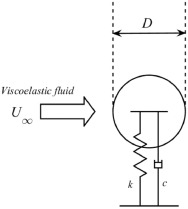
\includegraphics[width=4cm]{fig1.jpg}
    \caption{圆柱振荡模型}
    \label{fig:1}
\end{figure}

\section{研究模型}

在本研究中,采用任意拉格朗日-欧拉(ALE)方案来模拟圆柱体在粘弹性流体中由于振动而引起的边界运动。
具有空间均匀聚合物分子浓度的聚合物溶液的流体力学和粘弹性可以通过以下一组无量纲化方程来描述:
\newcommand*{\uu}[0]{\mathrm{u}}
\newcommand*{\cc}[0]{\mathrm{c}}
\newcommand*{\ts}[0]{{t^*}}
\begin{equation}
    \nabla \cdot \left(\right. u - u_{c} \left.\right) = 0
\end{equation}
\begin{equation}
    \frac{\partial u}{\partial t^{\star}} + \left[\right. \left(\right. u - u_{c} \left.\right) \cdot \nabla \left]\right. u = - \nabla p + \frac{1}{\text{Re}} \left[\right. \beta \Delta u + \frac{\left(\right. 1 - \beta \left.\right)}{\text{We}} \nabla \cdot \left(\tau\right)^{p} \left]\right.
\end{equation}
\begin{equation}
    \frac{\partial c}{\partial t^{\star}} + \left[\right. \left(\right. u - u_{c} \left.\right) \cdot \nabla \left]\right. c = \left(\right. \nabla u \left.\right) \cdot c + c \left(\left(\right. \nabla u \left.\right)\right)^{T} - \frac{\left(\tau\right)^{p}}{W e} + \kappa \Delta c
\end{equation}
其中,\(u\)是归一化为均匀入流速度\(U_\infty\)的二维速度矢量。
\(t^*\)是通过\(D/U_\infty\)对圆柱直径\(D\)进行无量纲化的时间。
\(u_c\)是移动网格的速度矢量,\(p\)是压力,\(\tau_p\)是聚合物应力,\(c\)表示平均聚合物结构张量,
其定义为端到端矢量的预平均二阶张量积。

为了描述粘弹性的程度,定义了Weissenberg数(\(We\)),
它是聚合物松弛时间尺度\(\lambda\)与特征变形速率\(U_\infty/D\)的乘积,
即\(We = \lambda U_\infty/D\)。
雷诺数(\(Re\))定义为\(\rho DU_\infty/(\mu_s + \mu_p)\),
其中\(\rho\)是密度,\(\mu_s\)是溶剂的粘度贡献,\(\mu_p\)是聚合物的粘度贡献。
参数\(\beta = \mu_s/(\mu_s + \mu_p)\)表示溶剂的零切变率粘度与总溶液的零切变率粘度之比。

为了改善数值模拟的稳定性,
在弹性应力输运方程的右侧引入人工扩散项\(\kappa \Delta c\)。
这里,\(\kappa\)被设定为相对较小的值。
本文将人工粘性的数值施密特数定义为\(Sc = \mu/\kappa\)。
在本研究中,给定的施密特数满足
\(Sc \approx O(10)\),
在最坏情况下,最小值被设定为8,以确保人工粘性对数值结果的影响很小。
在高Weissenberg数情况下,由于聚合物的延伸应力较高,人工粘性的扩散效应可能导致非平凡的定量差异。
然而,在相对较低的Weissenberg数下,通过保持合理的小数值施密特数,其对流动的影响是可接受的。

分子级的 FENE-P 模型被用于将稀溶性聚合物溶液中的单个聚合物分子近似为一根由有限可伸缩非线性弹簧连接的两个末端粒子组成的哑铃。
FENE-P 是应用于计算流体力学中的最佳聚合物模型之一,
因为它不需要在每个网格点上进行时间统计平均。
它已经证明能够捕捉到一些最重要的聚合物流动特性,如聚合物湍流阻力减小和剪切变薄。
通过对粒子施加的力的平衡,可以使用动力学理论确定聚合物应力 τp 的表达式 :
\begin{equation}
    \tau_p = cf(c) - I
\end{equation}
其中 Peterlin 函数为
\(f(c) = L^2 - \text{ND}L^2 - \text{Tr}(c)\),
这里的 \(L\) 是聚合物溶液中有限可伸缩非线性弹簧模型中的最大可伸长度。Tr 表示张量的迹。ND 表示流动的维数。

具有单自由度的广义结构模型可以表示如下:

\begin{equation}
    md^2y/dt^2 + cd(dy/dt) + ky = F_y(t)
\end{equation}

其中 \(y\) 是横向位移,\(t\) 是时间,\(F_y(t)\) 是作用在圆柱体上的横向力,\(m\)、\(c\) 和 \(k\) 分别表示圆柱体的质量、阻尼和弹簧常数。
由于位移和时间分别经过标准化,分别除以 \(D\) 和 \(D/U_\infty\),结构运动方程可以写成如下形式:
\begin{equation}
    d^2y^*/dt^{*2} + 4\pi\xi U_{\text{red}} dy^*/dt^* + 4\pi^2U_{\text{red}}^2y^* = \frac{2CL}{\pi m^*}
\end{equation}

其中 \(y^*\) 和 \(t^*\) 是相应的无量纲横向位移和时间。
\(U_{\text{red}}\) 是所谓的减速速度,它衡量了圆柱体惯性力与弹簧力之比的根。
它的定义为 \(U_{\text{red}} = U_\infty/f_nD\),其中 \(f_n = \frac{1}{2\pi}\sqrt{\frac{k}{m}}\)
是圆柱体的固有频率。\(m^* = \frac{4m}{\pi\rho D^2}\) 是相同体积中固体与
流体的质量比,\(C_L(t) = \frac{2F_y(t)}{\rho lU_\infty^2D}\) 和
\(\xi = \frac{c}{2\sqrt{km}}\)
分别是对应的升力和结构阻尼系数。

\section{数值方法}

为了耦合计算结构位移,
本文采用了一种流固松耦合方法来模拟非线性流固耦合问题。
该方法首先基于瞬时几何配置和粘弹性流体的控制方程获得流场,
然后将流体的力施加给结构运动方程。
接着,在相同物理时间步长内,通过状态空间方法,
基于一阶常微分方程的初值问题求解结构的位移。

流动方程和弹性应力输运方程之间的耦合是通过时间分裂在一个迭代步骤中实现的。
采用压力速度耦合算法来求解质量和动量方程,从而得到速度和压力的结果。
在每个时间步骤中,当残差收敛时,迭代停止。
通过上述时间步骤的迭代,可以获得流场对圆柱体的载荷。
然后,通过四阶龙格-库塔方法在同一步骤中更新圆柱体的位移方程,
以获得此时刻圆柱体的位置和速度。

圆柱体和网格的位置是通过求解网格系统的扩散方程来更新的。
在每个计算时间步骤之后,由于圆柱体的位移,计算域的边界发生变化。
有限元节点的位置相应地移动,通过求解修改后的拉普拉斯方程来实现:
\begin{equation}
    \nabla \cdot (\gamma \nabla S_y) = 0
\end{equation}
其中,$S_y$表示有限元单元节点在y方向上的位移,
$\gamma$是控制网格变形的参数。
为了确保在靠近圆柱体的小单元中扭曲很小,
有限元单元内的参数$\gamma$选择为$\gamma = 1/V^{1.5}$,
其中$V$是有限元单元的体积。使用基于ALE的有限体积法来处理移动界面。

通过有限体积法,获得控制方程的数值解,
其中偏微分方程转化为一组具有保守性质的离散代数方程。
采用QUICK方案对动量方程和弹性应力输运方程中的对流项进行离散化处理。
采用二阶中心差分格式对动量方程和弹性输运方程中的扩散项进行离散化处理。
然后更新网格,为下一个时间步骤做准备。
通过上述方法,本文得到流场计算和网格更新的组合算法。
速度场以均匀入流速度
初始化,弹性应力张量以单位张量初始化。

动量方程中弹性应力源项的散度是通过使用计算中最新的
结构张量$c_{ij}$的值来计算的。
这避免了对$\tau_{pij}$的边界的指定。
由于壁面是无穿透的,$c_{ij}$
可以被正确计算。
在当前的二维数值模拟中,可以写成如下形式:
\begin{equation}
    \frac{{\partial \tau_{pij}}}{{\partial x_j}} =
    \frac{{\partial}}{{\partial x_j}} \left[ (L^2-2)c_{ij}\frac{{L^2-c_{kk}}}{L^2}
    - \delta_{ij} \right] = (L^2-2)\left( \frac{{L^2-c_{kk}}}{{L^2}}
    \frac{{\partial c_{ij}}}{{\partial x_j}} \right) + \frac{{c_{ij}
            \frac{{\partial c_{kk}}}{{\partial x_j}}}}{{(L^2-c_{kk})^2}}
\end{equation}
\begin{figure}[H]
    \centering
    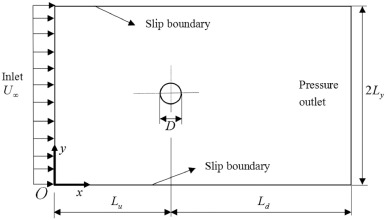
\includegraphics[width=8cm]{fig2.jpg}
    \caption{计算域设置}
    \label{fig:2}
\end{figure}
计算域的示意图如图\ref{fig:2}所示。
计算域在x方向和y方向分别为100D和50D。
圆柱体振动的自由度在y方向上。
入口边界条件设定为$u=1$和$v=0$,出口压力设定为零。
上下壁边界均设为滑移壁条件,圆柱体表面设为无滑移壁边界条件。
圆柱体最初固定在坐标$(25D, 25D)$处静止。在远场,弹性应力边界设置为$c=I$。
由于本构方程的双曲性质,壁面处的结构张量不需要给定边界条件。
然而,结构张量中的附加扩散项要求为张量提供必要的边界条件。在本工作中,
对于圆柱体壁法向的$c$实施无流条件。
图\ref{fig:3}显示了圆柱体附近的O型结构网格。
在更新网格时,可以确保网格的质量。
具体而言,最内部单元的厚度设置为0.005D。
为确保计算的稳定性,将时间步长设置得足够小,即$0.0025D/U_\infty$。

\begin{figure}[H]
    \centering
    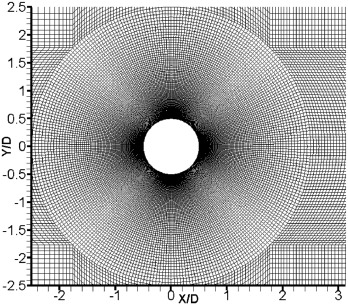
\includegraphics[width=8cm]{fig3.jpg}
    \caption{计算域设置}
    \label{fig:3}
\end{figure}

\section{数值验证}

为了评估目前的数值结果,
本文分别对静止圆柱体的粘弹性非定常尾流和圆柱体在牛顿流体中的涡激振动进行了独立的数值验证,
FENE-MCR是原始的Chicott-Rallison流体模型的修改模型,
假设模型中的$f(c)$与时间无变化。
这种简化可能会对非定常流动(如涡脱落尾流)产生一定误差,因为L不足够大。
但值得注意的是,这些FENE模型在L趋于无穷大时逼近于Oldroyd-B模型。
在Oldroyd-B模型中,$f(c)=1$,因此这种假设是合理的。
对于FENE-MCR流体,可以通过这种简化来解决弹性应力,无需解决结构张量。




\begin{table*}[htbp]
    \begin{center}
        \caption{Re = 100和L = 10时固定圆柱体在粘弹性流体和牛顿流体中的阻力系数比较}
        \label{tab:2}
        \begin{tabular}{cccccc}
            \hline
            We/Cd & 当前结果 & Richter et al. &        & Oliveira            \\
            \hline
                  & FENE-P   & FENE-MCR       & FENE-P & FENE-MCR & FENE-MCR \\
            0     & 1.361    & 1.361          & 1.343  & 1.343    & 1.3701   \\
            0.5   & 1.362    & 1.368          & 1.351  & 1.374    & 1.3795   \\
            1     & 1.363    & 1.359          & 1.346  & 1.363    & 1.3732   \\
            2     & 1.34     & 1.338          & -      & -        & 1.3527   \\
            3     & 1.321    & 1.324          & 1.302  & 1.339    & 1.3386   \\
            4     & 1.304    & 1.314          & -      & -        & 1.3296   \\
            5     & 1.293    & 1.305          & 1.277  & 1.323    & 1.3235   \\
            10    & 1.265    & 1.296          & 1.25   & 1.307    & 1.3098   \\
            20    & 1.246    & 1.289          & 1.233  & 1.298    & 1.3022   \\
            40    & 1.233    & 1.286          & 1.222  & 1.294    & 1.2983   \\
            80    & 1.227    & 1.285          & 1.216  & 1.291    & 1.2962   \\
            \hline
        \end{tabular}
    \end{center}
\end{table*}

\begin{table*}[htbp]
    \begin{center}
        \caption{Re = 100和L = 10时固定圆柱体后方涡脱落的St数比较}
        \label{tab:3}
        \begin{tabular}{cccccc}
            \hline
            We/St  & 当前结果 & Richter et al. &        & Oliveira            \\
            \hline
                   & FENE-P   & FENE-MCR       & FENE-P & FENE-MCR & FENE-MCR \\
            We = 0 & 0.1669   & 0.1669         & 0.1677 & 0.1669   & 0.167    \\
            0.5    & 0.1658   & 0.1659         & 0.1657 & 0.1649   & 0.1659   \\
            1      & 0.1645   & 0.1646         & 0.1641 & 0.163    & 0.1644   \\
            2      & 0.1625   & 0.1625         & -      & -        & 0.162    \\
            3      & 0.1610   & 0.1613         & 0.1603 & 0.1586   & 0.1605   \\
            4      & 0.1601   & 0.1606         & -      & -        & 0.1597   \\
            5      & 0.1593   & 0.1602         & 0.1585 & 0.1571   & 0.1591   \\
            10     & 0.1582   & 0.1594         & 0.1569 & 0.1557   & 0.1579   \\
            20     & 0.1584   & 0.1594         & 0.1566 & 0.1551
                   & 0.1575                                                   \\
            40     & 0.1592   & 0.1599         & 0.1569 & 0.1547   & 0.1576   \\
            80     & 0.1596   & 0.1601         & 0.1576 & 0.1547   & 0.1578   \\
            \hline
        \end{tabular}
    \end{center}
\end{table*}

在粘弹性涡脱落流动的验证中,本文采用了Oliveira的研究中的Mesh 3。
所有参数与Oliveira和Richter等人的先前研究相同。
阻力系数和St数分别在Re = 100和L = 10时列在表\ref{tab:2}和表\ref{tab:3}中。
显然,本文的结果与Oliveira和Richter等人[25]的结果非常一致。
FENE-MCR流体的阻力减小差异小于1.5\%。
对于FENE-P流体,可以观察到在低We值时差异比较轻微,
并随着Weissenberg数增加到80而增大约5\%。
St数的差异也呈现相同的行为。
总之,所有的数值结果在低Weissenberg数下都非常一致,
并在高Weissenberg数下表现出相同的物理行为,尽管在We = 80时误差略微增加约3\%。

此外,本文提取了一些流场细节与Richter等人进行了比较。
图\ref{fig:4}显示了在Re = 100,We = 10和L = 100时圆柱体壁前的弹性应力分布。
对于更高的最大聚合物可伸展性和更高的Weissenberg数,
流场在离开物体的前方显示出固体的趋势,
其特征为高弹性应力、高压力和流速降低。
值得注意的是,
目前的Weissenberg数和最大聚合物可伸展性L = 100在数值上是相当高的。
沿着中心线的平均结构张量迹的剖面表明,
本文的数值结果与文献中的结果一致,
如图\ref{fig:4}所示。最大尾迹的误差约为2\%,
表明目前的结果在数值扩散方面存在轻微问题。

\begin{figure}[H]
    \centering
    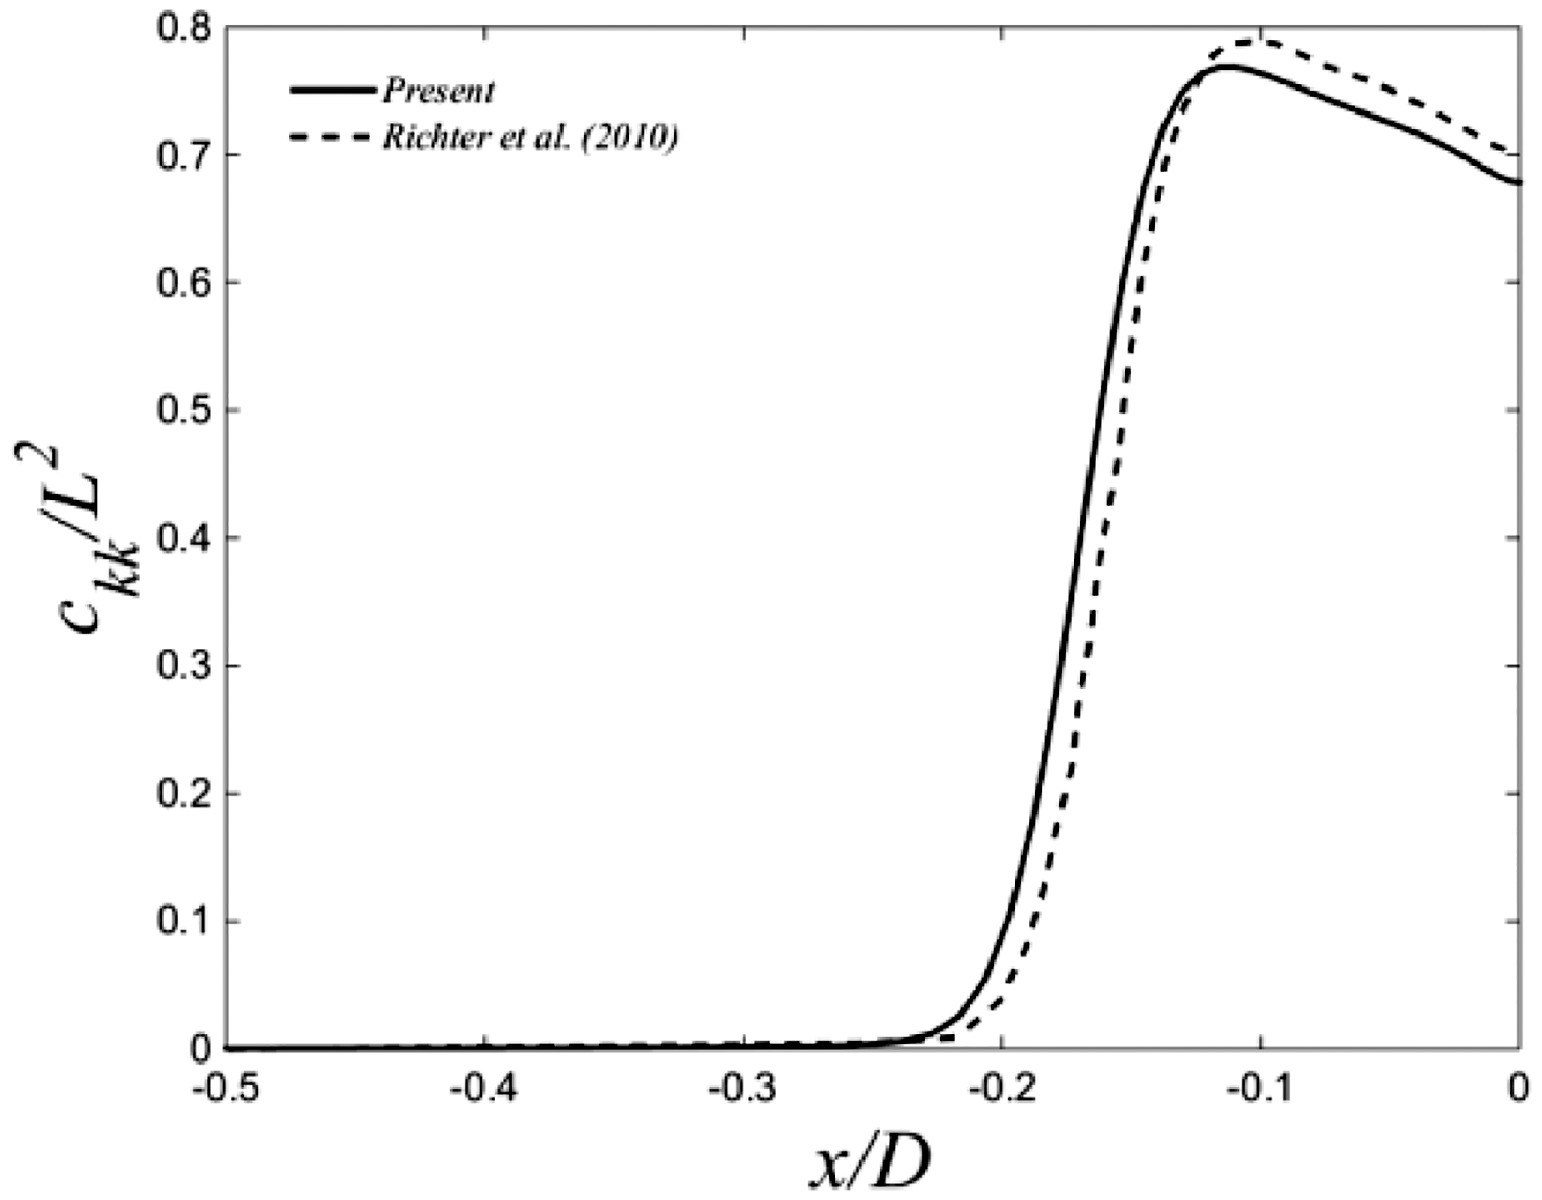
\includegraphics[width=11cm]{fig4.jpg}
    \caption{
        圆柱前缘附近的弹性张量对比}
    \label{fig:4}
\end{figure}


\section{结果与分析}

\subsection{粘弹性对VIV的影响}

\begin{figure}[H]
    \centering
    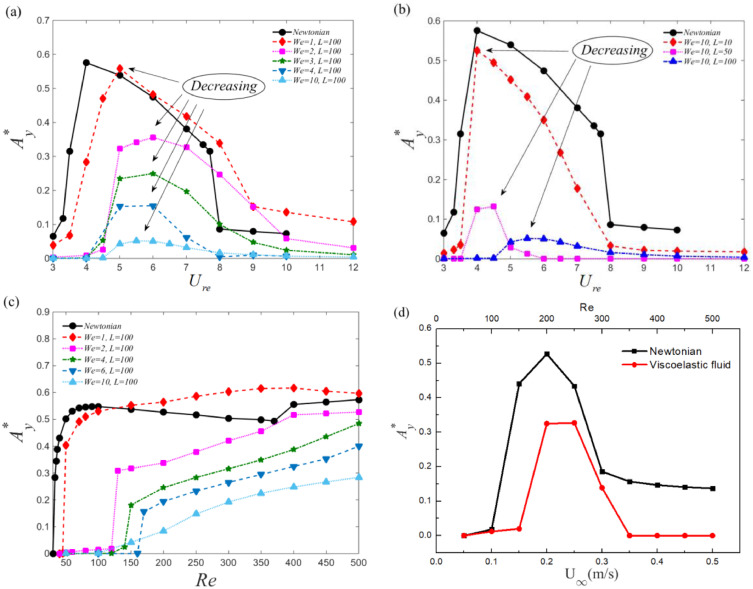
\includegraphics[width=11cm]{fig6.jpg}
    \caption{
        (a) 对于不同的Weissenberg数,振幅的最大值随减速速度的变化情况;
        (b) 对于不同的最大聚合物可伸展性,振幅的最大值随减速速度的变化情况;
        (c) 在固定的减速速度4.92下,振幅的最大值随雷诺数的变化情况;
        (d) 在不同的入流速度下,牛顿流体和选择的粘弹性流体的振幅的最大值进行比较。}
    \label{fig:6}
\end{figure}

图\ref{fig:6}(a)显示了在雷诺数为150时,
单自由度圆柱体在恒定L = 100条件下的振幅最大值与减速速度的关系。
从这些比较中可以看出,随着Weissenberg数的增加,
圆柱体的振幅总体上减小。
在We = 10时,可以看到振幅最大值仅为0.0516D,
约为牛顿流体中的10\%,
大约发生在Ure = 5.5。
对于粘弹性流体的另一个特点是最大振幅的峰值向更大的减速速度移动。
图\ref{fig:6}(b)显示了在We = 10时,Re = 150
下不同最大聚合物可伸展性下最大振幅与减速速度的关系。
对于We = 10和L = 50,最大振幅出现在Ure = 4.5处,
相应的振幅约为0.146D,
为牛顿流体中的25\%。
结合图\ref{fig:6}(a)和6(b),
可以看出较大的最大可伸展性会导致振幅的减小。
这与较大的最大可伸展性会产生更大的弹性效应,
并且更多的动能转化为储存在聚合物分子中的弹性能量有关。


在牛顿流体中,低雷诺数下的VIV可以引发流场的不稳定性,
这在文献中得到了广泛报道。
Kou等人在Ure∼Re空间中给出了质量比为4.73的一度VIV的最小雷诺数约为19.7。
这个临界雷诺数远小于47.5,
后者是静止圆柱体后的涡脱落的临界雷诺数。
在本文的模拟中,对于给定质量比的牛顿流体,
结构在雷诺数约为31和减速速度4.92时开始振动,
如图\ref{fig:6}(c)所示。而对于We = 2和L = 100,
结构的振动发生在雷诺数为40时。
随着Weissenberg数增加到4和6,
相应的临界雷诺数分别增加到50和80。
也就是说,聚合物的添加可以改变结构振动的临界雷诺数。
这类似于粘弹性流体在静止圆柱体上的流动。
Sahin和Owens 在Re∼We空间中发现了FENE-MCR(L = 100)
流体的圆柱体尾流流动不稳定性的最大临界雷诺数为68.65。

当Weissenberg数小于10时,
图\ref{fig:6}(c)中存在一个振幅突变区域,
其中振幅随雷诺数的变化发生剧烈变化。
对于牛顿流体,
振幅在雷诺数为31时为零,
而在雷诺数为33时,最大振幅增加到0.284D。
对于We = 1和L = 100,
振幅在雷诺数为45时为0.0004D,
而在雷诺数为50时振幅增加到0.403D。
振幅的这种剧烈增长表明,
当雷诺数大于临界值时,相
对于牛顿流体,
振幅对减速速度的敏感性高于对雷诺数的敏感性。
然而,雷诺数对振幅的最大影响在较高的Weissenberg数案例中更为显著。
如图\ref{fig:6}(c)所示,对于雷诺数200,
圆柱体在牛顿流体中的最大振幅为0.526D。
但是对于We = 2和L = 100,
结构的最大振幅为0.338D。
对于We = 10和L = 100,结构的最大振幅仅为0.084D,振动
减小与牛顿流体相比高达84\%。
通过这些比较,本文可以观察到聚合物的添加可以显著降低
在给定减速速度Ure = 4.92下的振动。
还注意到,微小的添加也可以略微增强振动,
例如We = 1和L = 100。

为了进一步评估粘弹性流体对VIV的影响,
本文还以实验的风格呈现了结果,
该方式保持流体和结构的恒定性质,
并增加了入流速度。
随着入流速度的增加,诸如雷诺数、
减速速度和Weissenberg数等参数同时增加。
这种方法有助于根据直觉观察粘弹性流体的影响,它便于与实验结果进行比较。
在这里,本文进行了粘弹性流体的模拟,松弛时间为10ms,
相应的PEO浓度约为0.75 × 10−3\%质量分数,
其分子量为350万。
圆柱体直径设定为1mm,
入流速度范围从0.05到0.5m/s,以
观察牛顿流体和粘弹性流体之间的差异。
如图\ref{fig:6}(d)所示,与牛顿流体相比,
粘弹性流体中的振动最大振幅明显降低。
此外,它表明为了观察到非平凡的VIV,
粘弹性流体中的流速应高于牛顿流体。
这与以前观察到的粘弹性流体可以抑制VIV并增加启动减速速度的结果一致。

\begin{figure}[H]
    \centering
    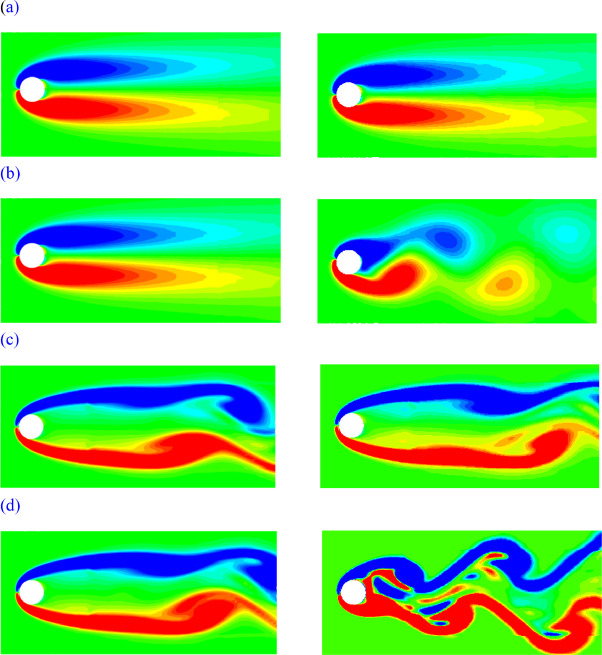
\includegraphics[width=8cm]{fig7.jpg}
    \caption{
        Ure = 4.92时的涡量图,
        其中(a)代表Re = 30的牛顿流体,
        (b)代表Re e= 33的牛顿流体,
        (c)代表We = 6、L = 100时的Re = 160的粘弹性流体,
        (d)代表We = 6、L = 100时的Re = 170的粘弹性流体。左侧为静止的圆柱体,右侧为振动的圆柱体。
    }
    \label{fig:7}
\end{figure}

图\ref{fig:7}中绘制了牛顿流体和粘弹性流体中VIV的涡量,
以检查尾迹模式。
对于静止圆柱体的尾迹,
先前的研究已经报告了在相同雷诺数下牛顿流体和粘弹性流体之间的差异。
Oliveira指出FENE-MCR流体可以增加形成长度并减弱涡旋。
类似的行为也观察到其他粘弹性流体,
如Oldroyd-B和FENE-P流体。
图\ref{fig:7}(a)和
图\ref{fig:7}(b)分别绘制了在减速速度4.92下的牛顿流体的尾迹形成,
其中Re = 30和Re = 33。
在牛顿流体中,Re = 30时流动是稳定的。
当Re = 33时,振动由涡旋引起,
可以在尾迹中观察到两个交替涡旋的卷起。
如图\ref{fig:6}(a)所示,
Re = 33时圆柱体的响应振幅高达0.284D。
对于We = 6和L = 100的粘弹性流体,
在Re = 160和Re = 170时的尾迹模式如
图\ref{fig:7}(c)(d)所示。
与牛顿流体类似,
Re = 160时圆柱体响应的振幅非常小。
可以观察到分离的剪切层卷起并在圆柱体后方更远处形成新的横向涡旋
[图\ref{fig:7}(c)]。
这种现象已经在由于聚合物添加引起的静止圆柱体尾迹中观察到。
当雷诺数增加到170时,圆柱体的振幅较高,
剪切层卷起并在靠近圆柱体的地方形成新的横向涡旋。
此外,相干涡旋明显与牛顿流体中的脱落涡旋不同。
上下涡旋明显分层并沿着流动方向显著拉伸,
类似于图\ref{fig:7}(c)。
换句话说,当圆柱体在粘弹性流体中振动时,保持了固定圆柱体尾迹流动的涡旋特征,
例如涡旋沿流动方向的拉伸。与此同时,VIV可以在粘弹性流体中扩大尾迹流动的横向不稳定性。


\begin{figure}[H]
    \centering
    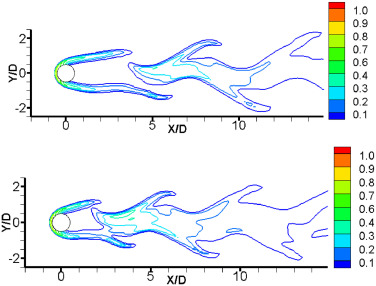
\includegraphics[width=11cm]{fig8.jpg}
    \caption{
        聚合物拉伸场:聚合物构型张量的迹。
        在Ure = 4.92条件下,
        比较静止圆柱体(上)和单自由度圆柱体(下),
        在Re = 150,We = 10和L = 100。
    }
    \label{fig:8}
\end{figure}

聚合物结构张量c的迹可以指示流体中聚合物的拉伸程度。
图\ref{fig:8}显示了在Ure = 4.92,Re = 150,We = 10和L = 100条件下,
对于静止圆柱体和振动圆柱体,
聚合物迹c的图,经过L2归一化。
在这个Weissenberg数下,由于聚合物的加入,
静止圆柱体的尾迹振动非常微弱。
很明显,聚合物在圆柱体周围被明显拉伸(图\ref{fig:8}上)。
实验证明(Cadot and Lebey ),
数值模拟也证实,
随着聚合物可伸长性的增加,静止圆柱体后方的环流区域显著延长。
对于具有单自由度的柔性圆柱体,
圆柱体响应振幅仍然在5-6.5的减速速度范围内保持在0.04D以下。
随着圆柱体的振动,尾迹中的聚合物拉伸相比静止圆柱体会减弱(图\ref{fig:8}下)。

\begin{figure}[H]
    \centering
    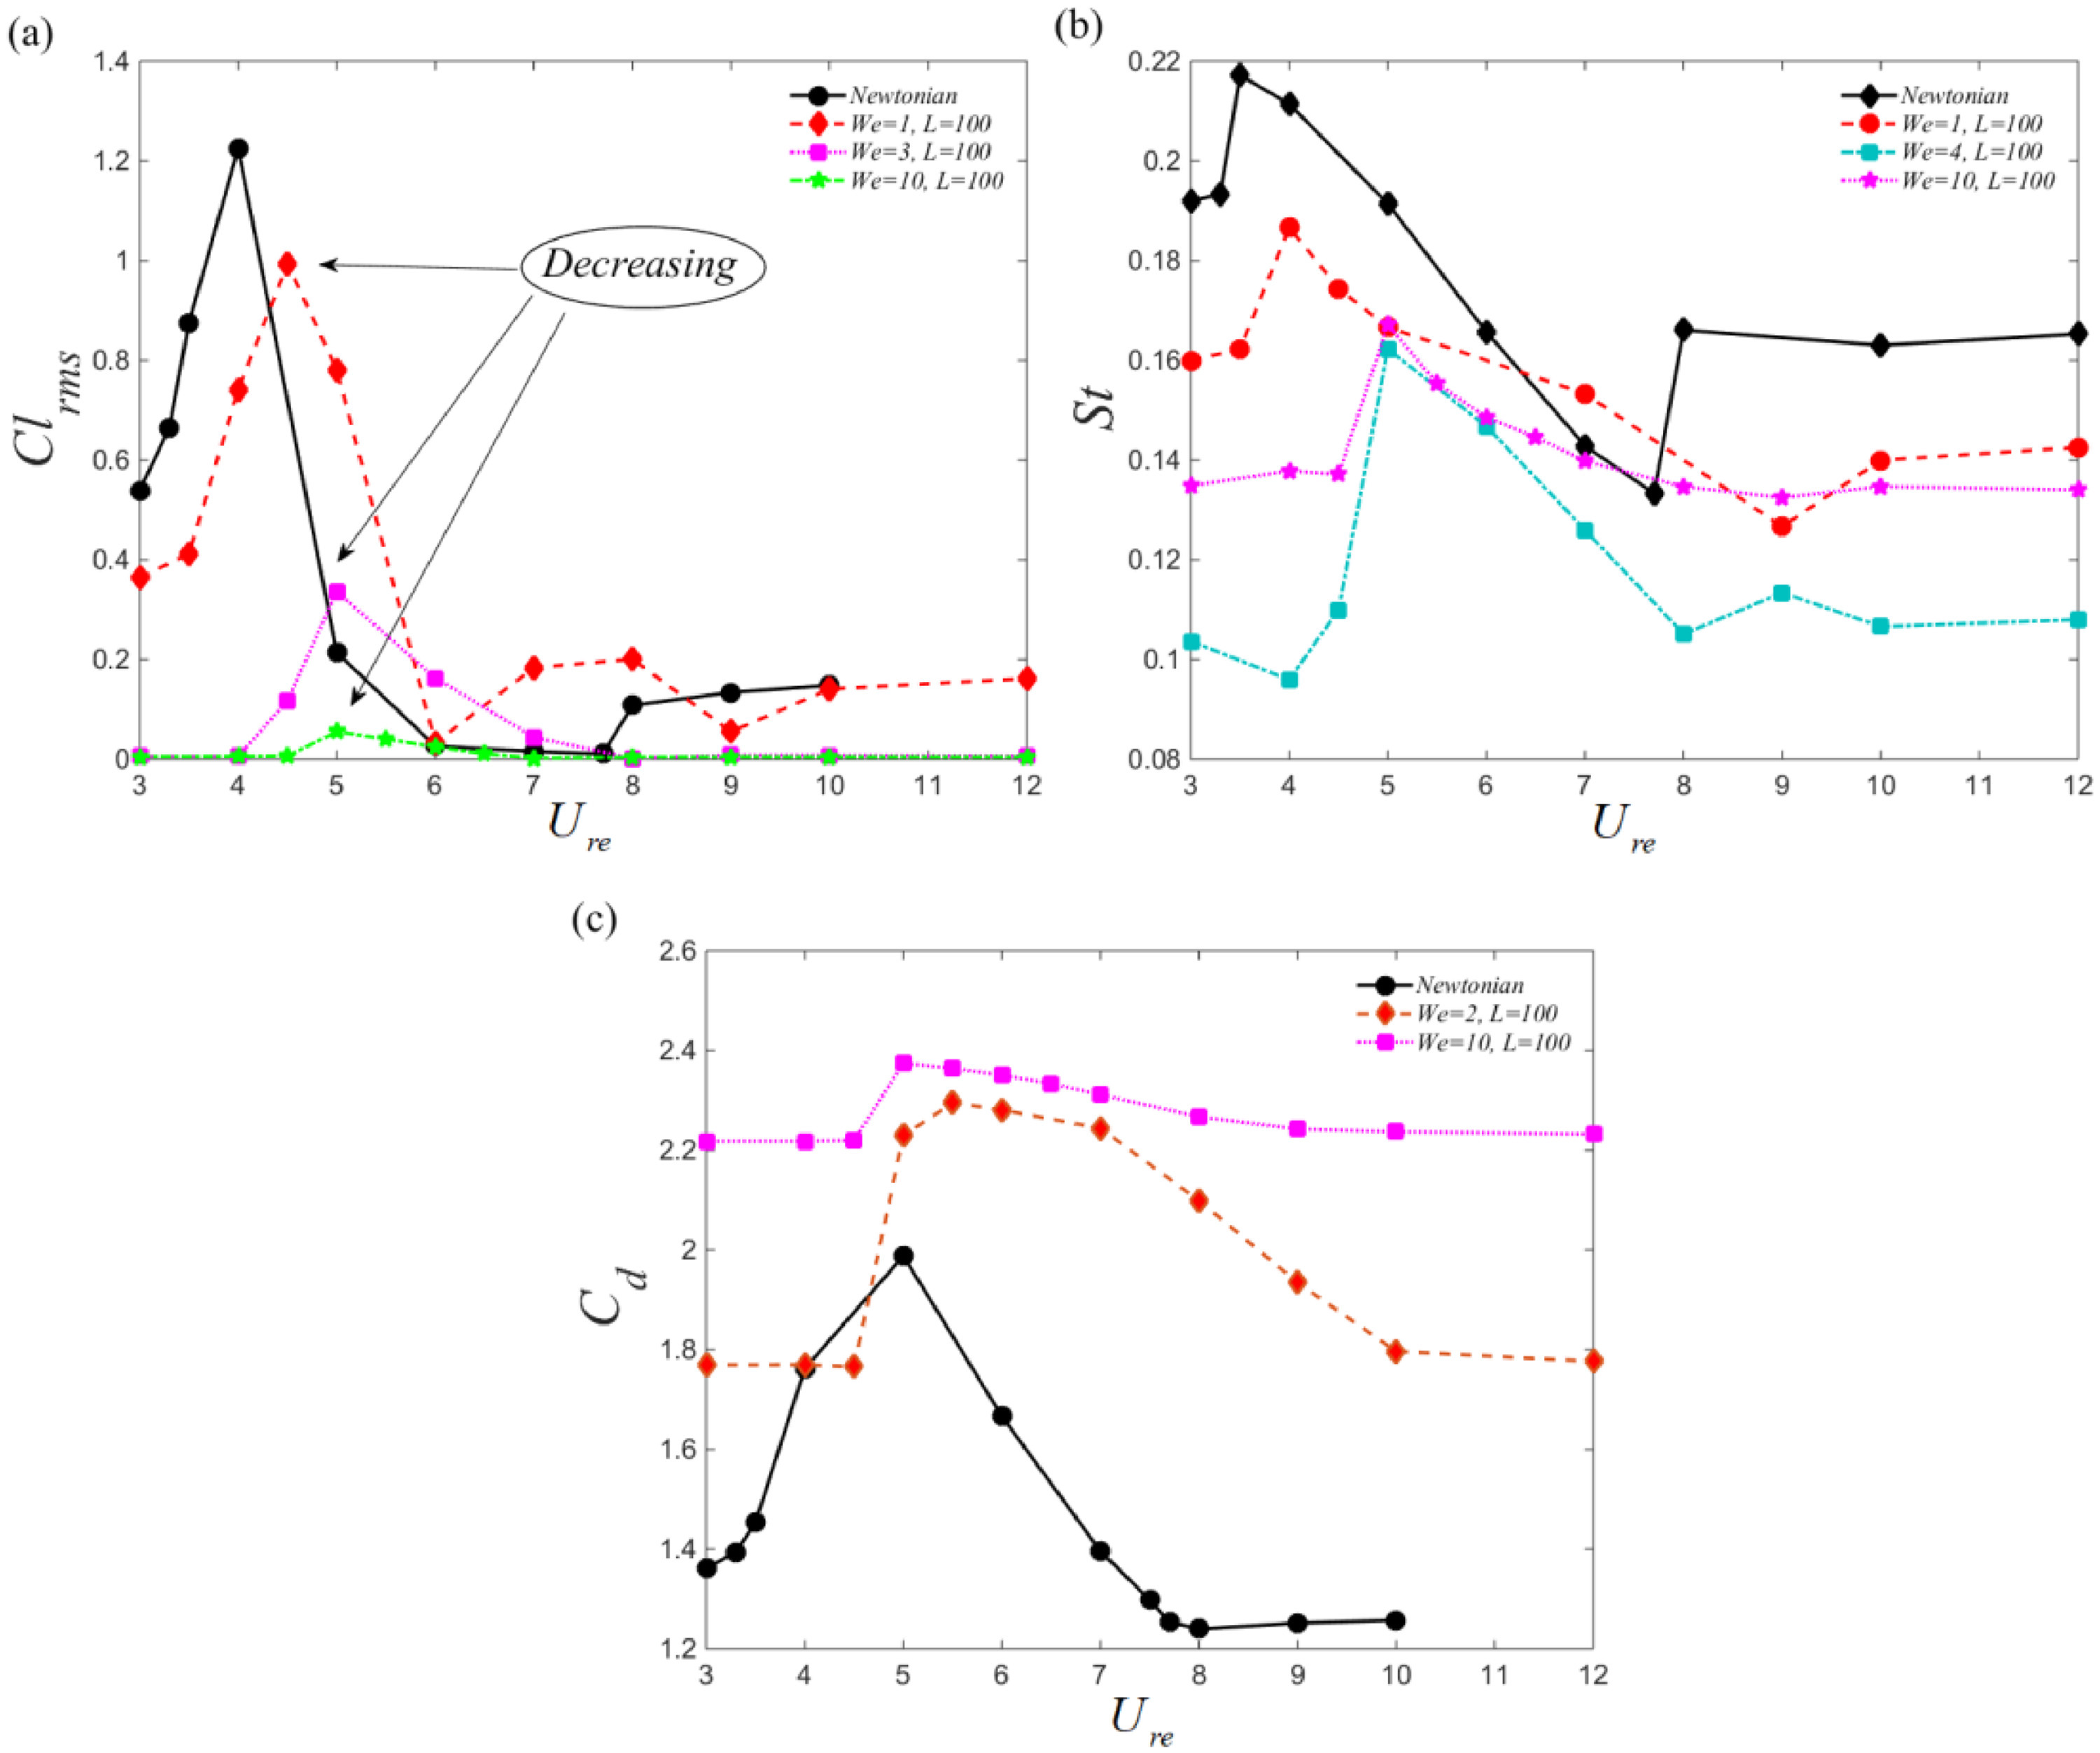
\includegraphics[width=12cm]{fig9.jpg}
    \caption{
        在雷诺数为150时,
        均方根升力系数(a)、
        St(b)以及时间平均阻力系数(c)与减速速度在不同Weissenberg数下的关系
    }
    \label{fig:9}
\end{figure}

图\ref{fig:9}(b)展示了在不同Weissenberg数下,
雷诺数为150时St数与减速速度之间的关系。
实际上,在Ure = 3的情况下,
圆柱体在牛顿流体和聚合物溶液中只以较小振幅振动[参见图\ref{fig:6}(a)]。
因此,流场的特征与流过静止圆柱体的流动非常接近。
显然,St数随着Weissenberg数的增加而先减小,
然后增加,对于Ure = 3这一结果与Usui等人在100≤Re≤300范围内进行的不同浓度PEO溶液实验非常吻合。
值得注意的是,圆柱体的振动是由流动的振动引起的。
在锁定区域内,通过添加聚合物,St数减小。
这导致最大振动幅度出现的减速速度在聚合物溶液中向更大值偏移,
如图\ref{fig:6}(a)所示。但对于We = 10,流场的St数大于We = 4的情况。
最大振动幅度的减速速度并没有向更大值偏移。要理解这个结果,
需要考虑在We = 10时流动的振荡非常弱,
这导致流体和固体之间的耦合也很弱。
这类似于质量比较高时的涡振动。
对于这种系统,涡脱落频率fs接近弹簧-质量系统的固有频率fn。
作用在圆柱体上的振动载荷太轻微,无法使结构振动。

\begin{figure}[H]
    \centering
    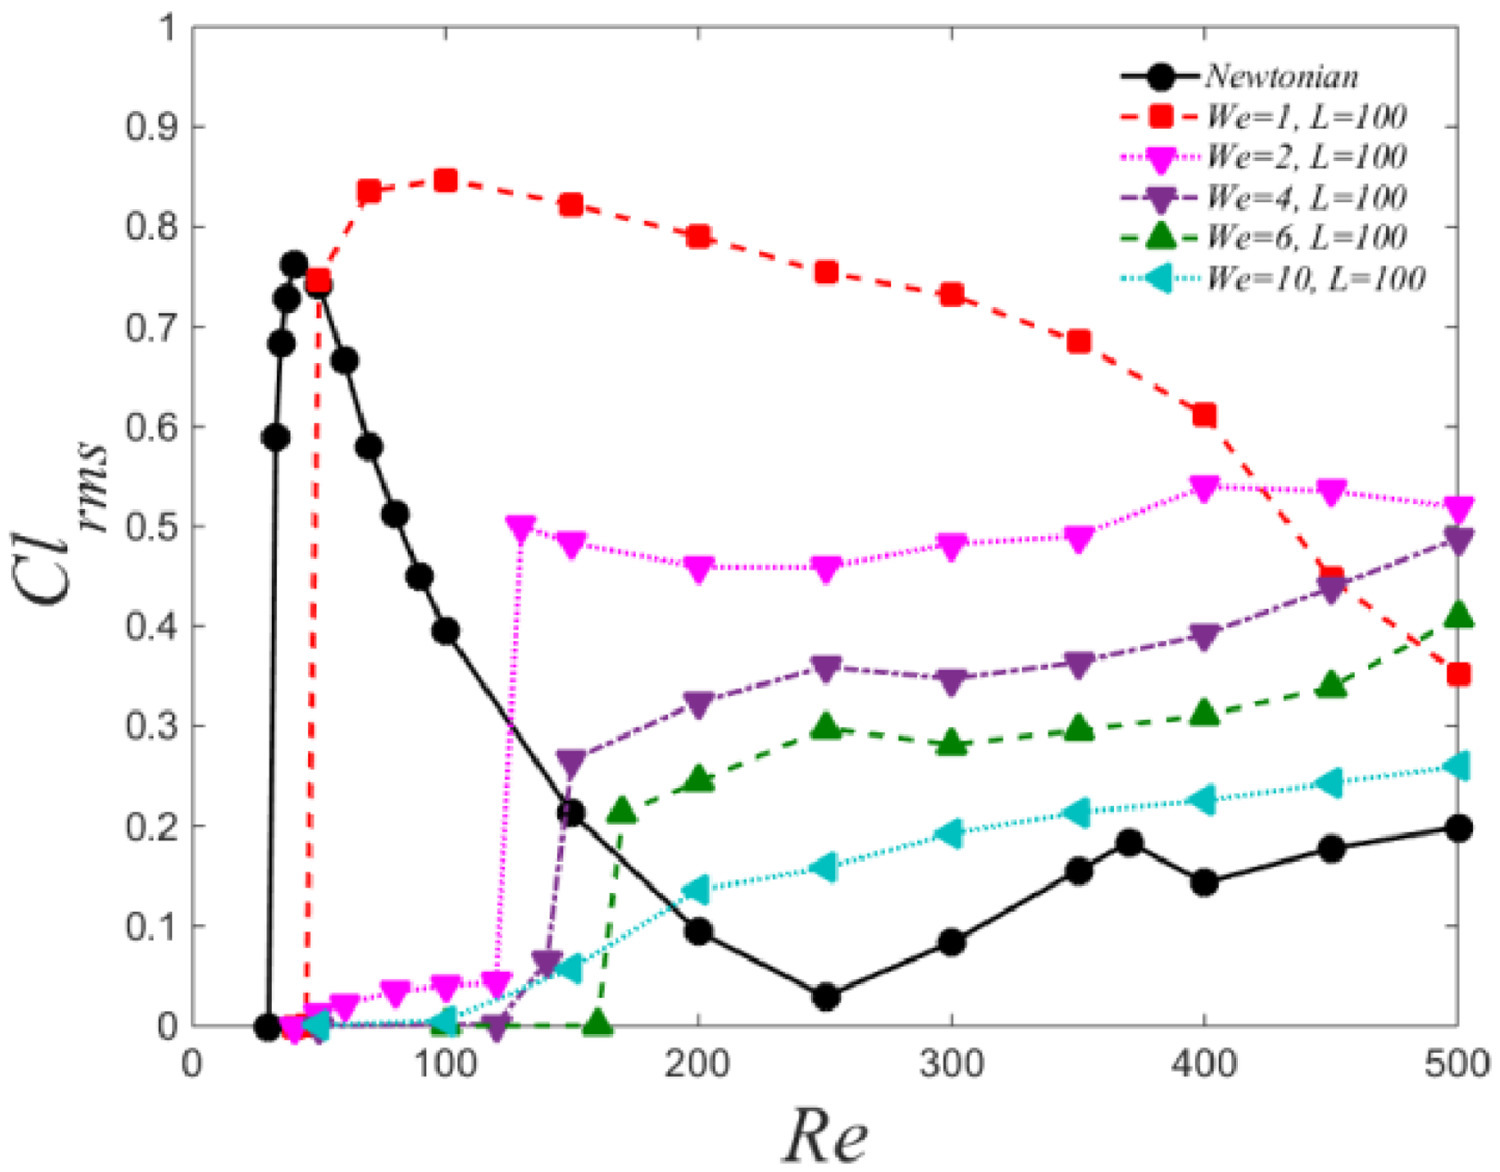
\includegraphics[width=11cm]{fig10.jpg}
    \caption{
        不同雷诺数和Weissenberg数下,减速速度为4.92时的均方根升力系数
    }
    \label{fig:10}
\end{figure}

事实上,振动幅度不仅与升力力量有关,
还与流体的阻力有关。当圆柱体强烈振动时,
它倾向于具有更大的阻力系数。
图\ref{fig:9}(c)描述了在雷诺数为150、不同Weissenberg数下,
阻力系数与减速速度之间的关系。
从图中可以看出,阻力系数在减速速度约为5处达到最大值
牛顿流体中的最大均方根阻力系数约为1.988。对于聚合物溶液,
本文仍然可以发现阻力系数在减速速度较大的振动幅度出现的位置达到最大值。
例如,We = 10的聚合物溶液在减速速度约为5时出现最大阻力系数,
振动幅度为0.0424D。值得注意的是,在当前雷诺
数150下,相对于静止圆柱体,
聚合物溶液中的圆柱阻力增加。
本文的模拟结果显示,We = 10时的平均阻力系数约为2.22,
而牛顿流体中静止圆柱体的阻力系数为1.362。
在较高的Weissenberg数下,
如前所述,流场与结构之间的耦合变得较弱,
而由于圆柱体的振动不如其牛顿流体对应物那样高,
阻力增加。
具体来说,可以看出We = 10自由振动圆柱体的最大平均阻力系数约为2.375。
与流过静止圆柱体相比,额外阻力差异仅为0.155,远小于牛顿流体中的0.748差异。

图\ref{fig:10}显示了在不同雷诺数下,
牛顿流体和聚合物溶液中的RMS升力系数。
在模拟中,牛顿流体的最大RMS升力系数约为40左右的雷诺数,
然后随着雷诺数的增加,RMS升力系数降至相对较低的水平。
这与Singh和Mittal 的研究结果一致。
对于We = 1的聚合物溶液,RMS升力系数在50-400的雷诺数范围内保持在0.6以上,
这导致了如图\ref{fig:6}(c)所示的高振幅振动。
但对于We≥2,当雷诺数大于临界值时,RMS升力系数随雷诺数的增加略有变化。
这种现象对应于图\ref{fig:6}(c)中振幅突然增加的情况
。
在这个阶段,RMS升力系数随着Weissenberg数的增加而减小,从而振幅减小。

\begin{figure}[htbp]
    \centering
    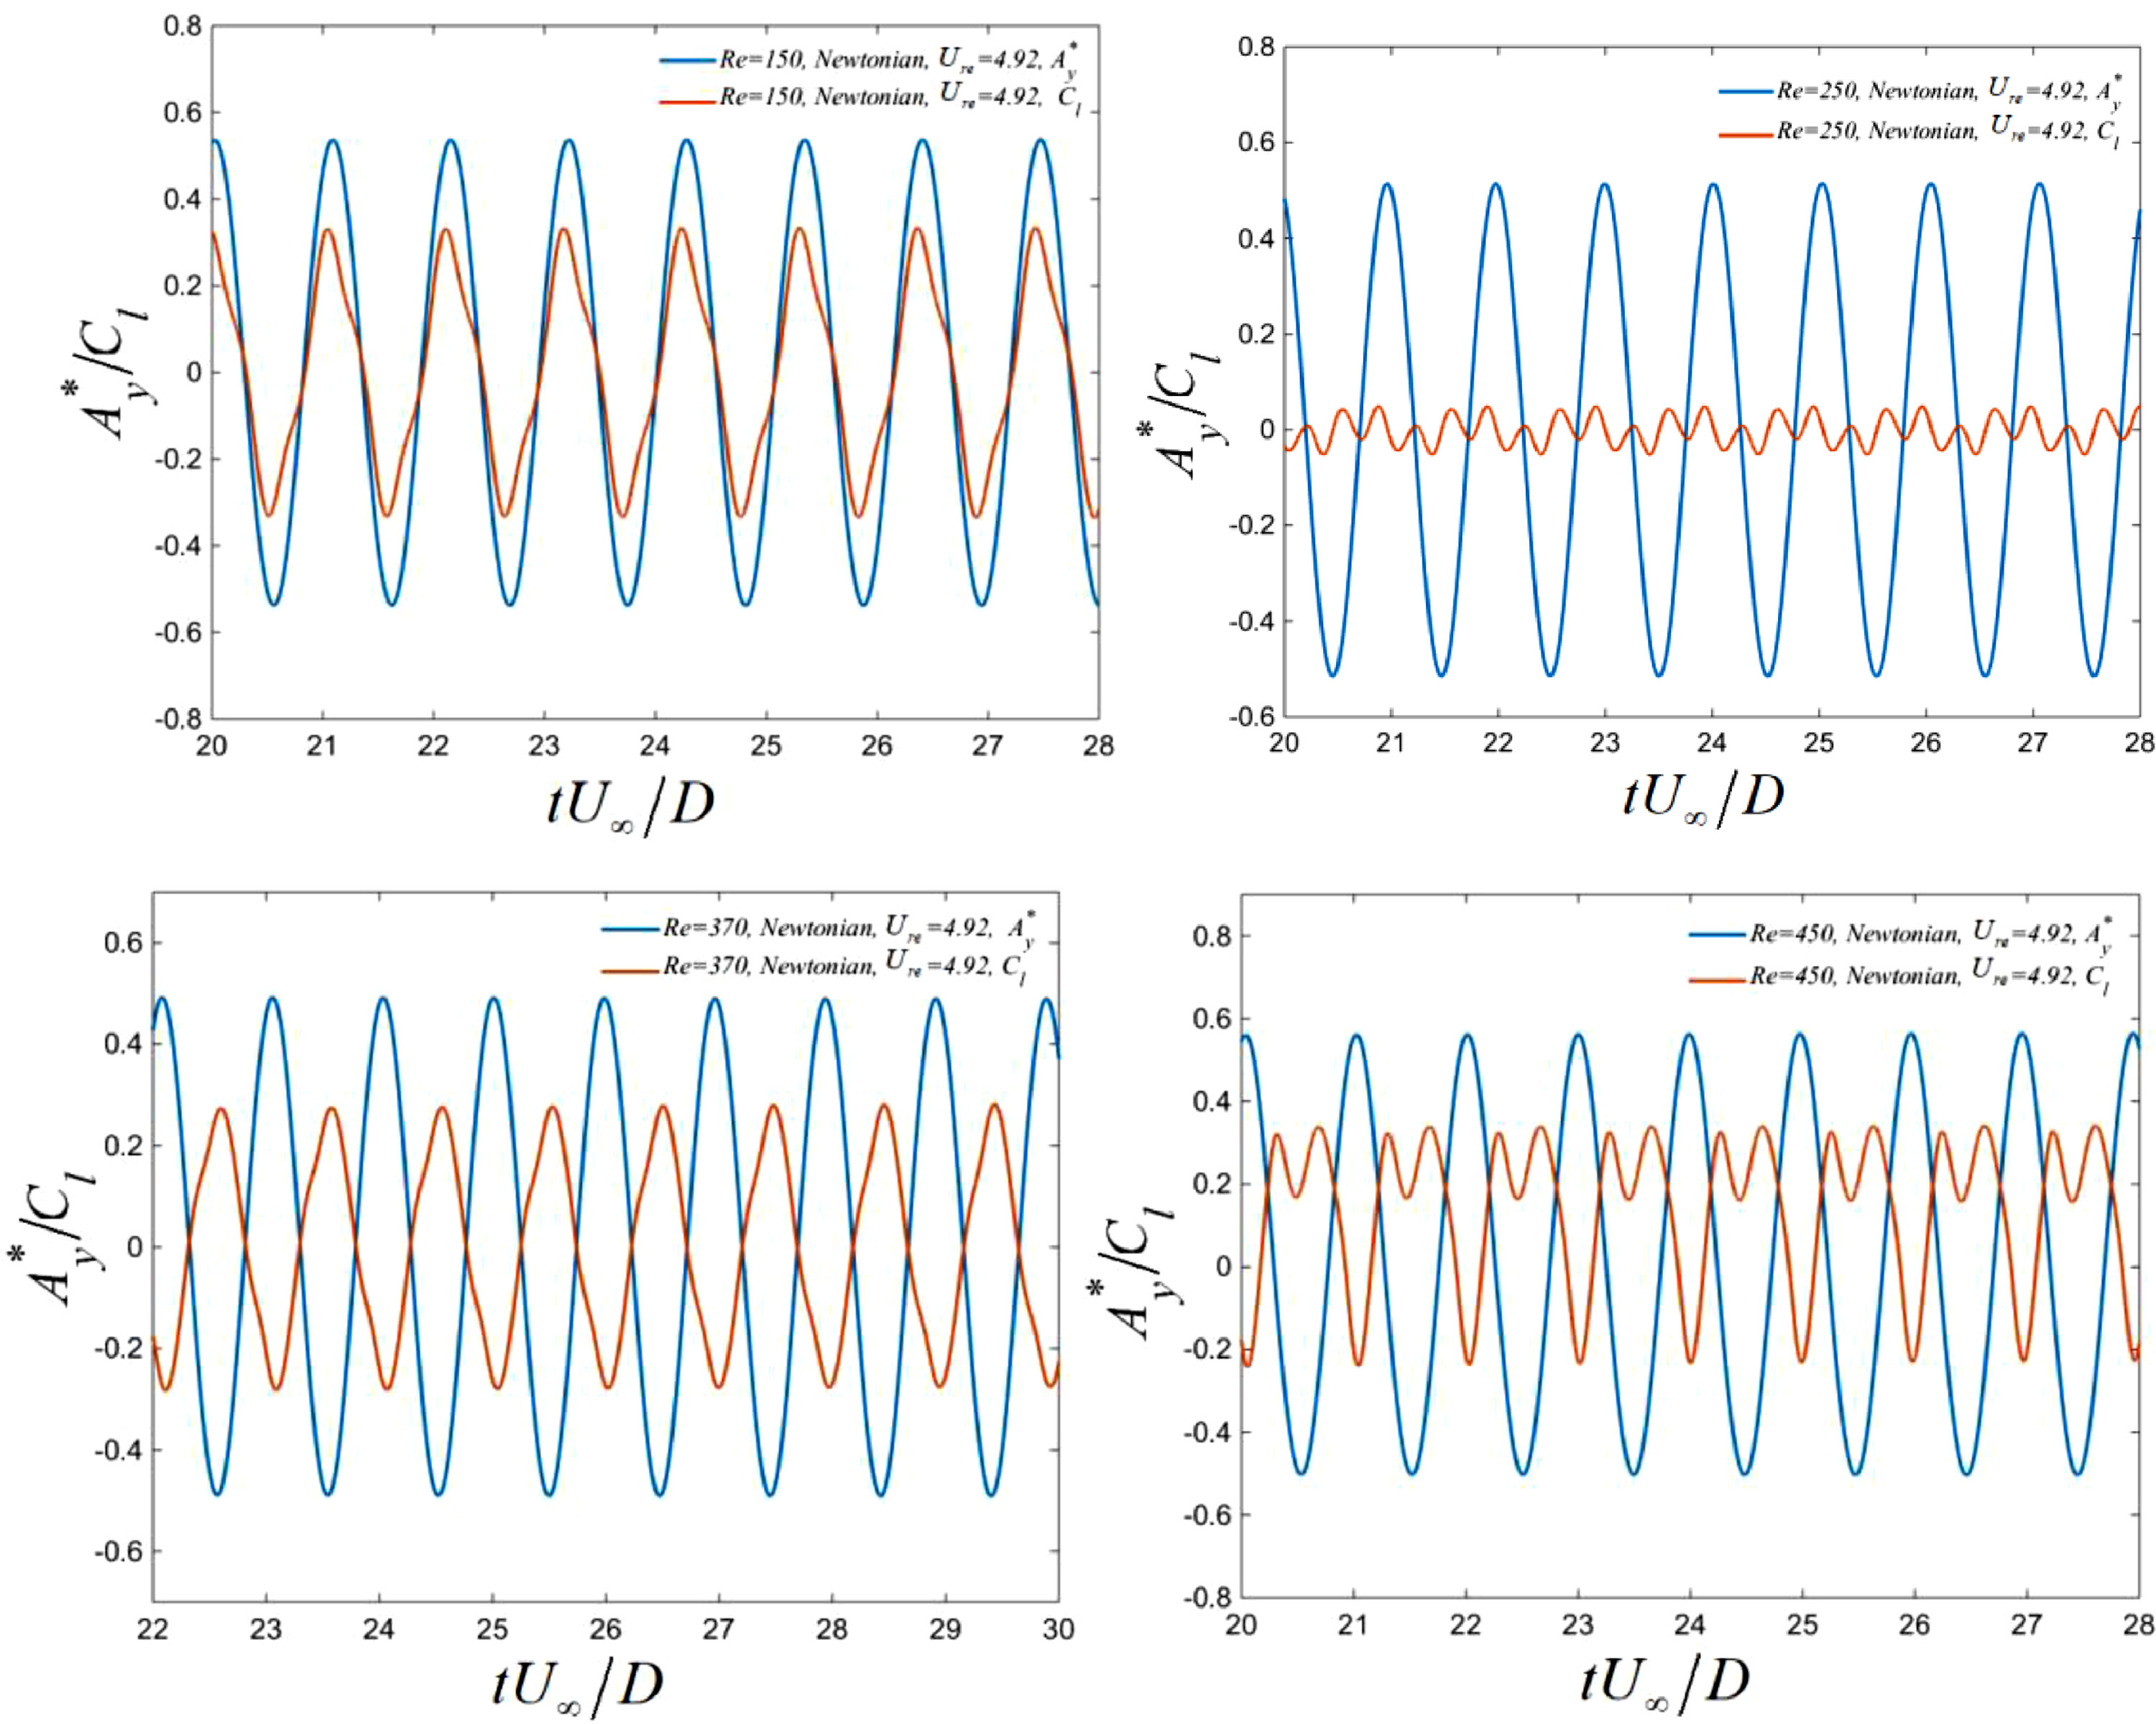
\includegraphics[width=11cm]{fig11.jpg}
    \caption{
        牛顿流体在不同雷诺数下圆柱振动幅度和升力系数的时间历史
    }
    \label{fig:11}
\end{figure}

\begin{figure}[htbp]
    \centering
    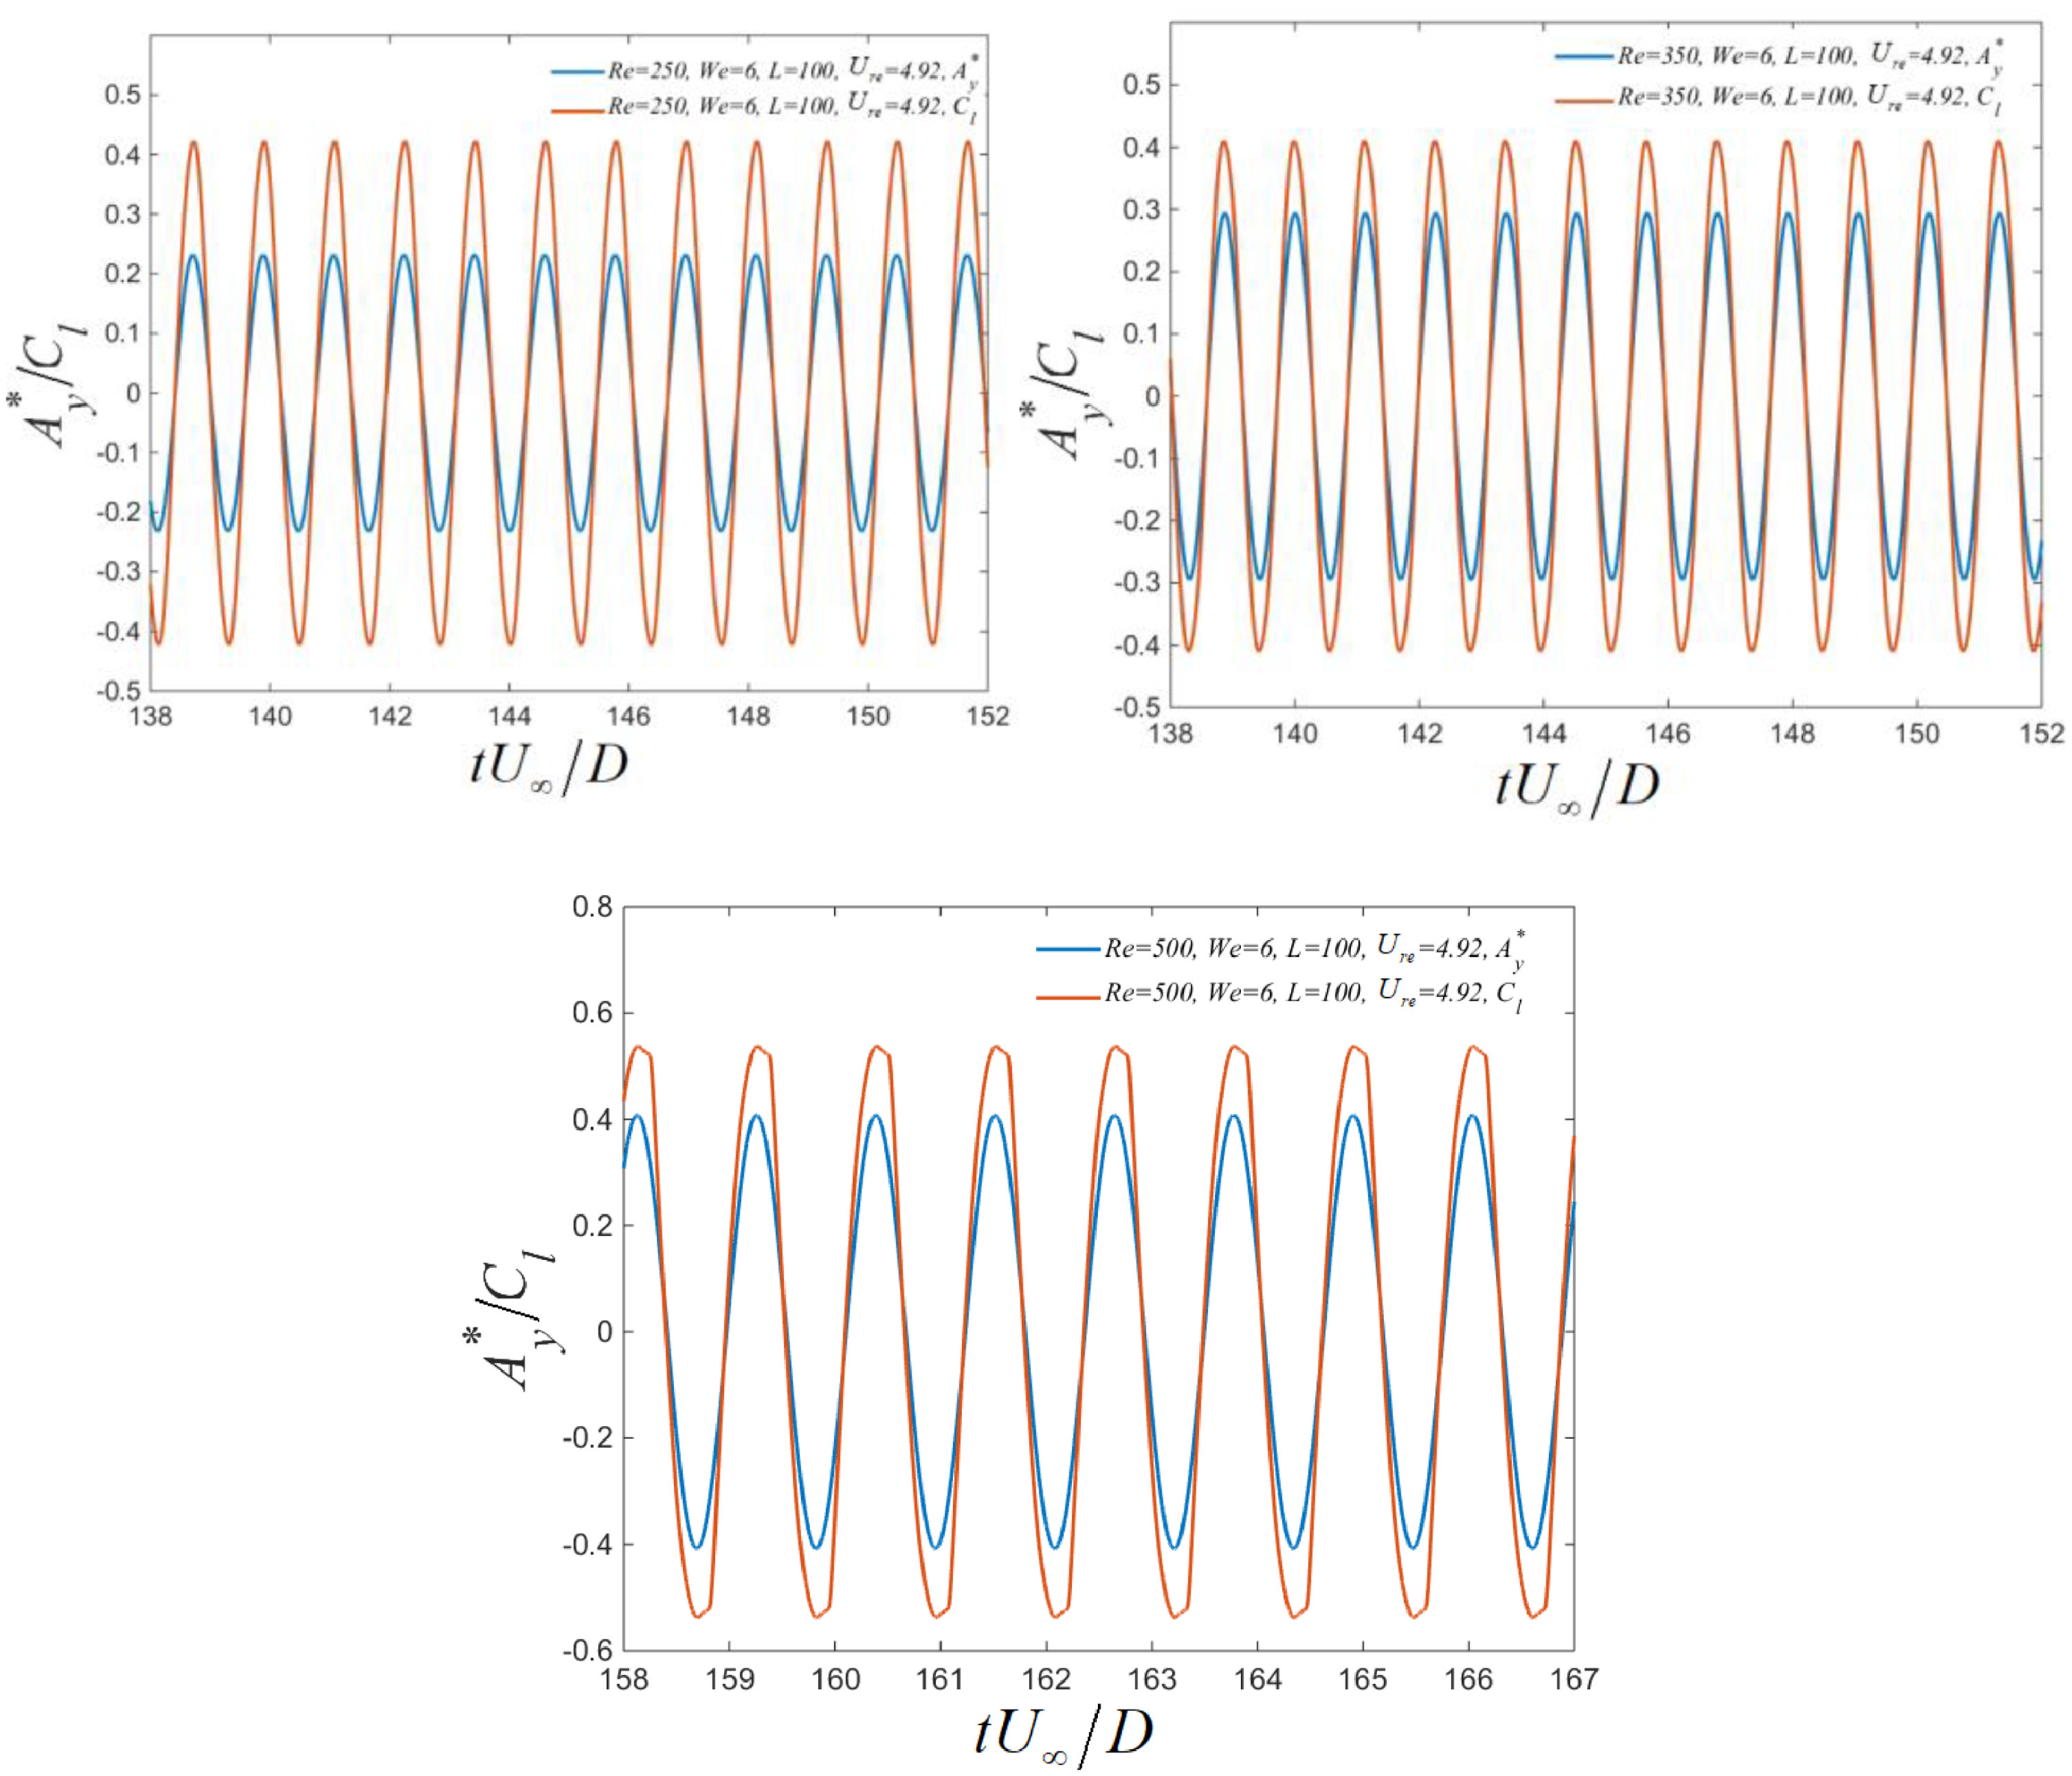
\includegraphics[width=11cm]{fig12.jpg}
    \caption{
        粘弹性流体中不同雷诺数下圆柱振动和升力系数的时间历史
    }
    \label{fig:12}
\end{figure}

\begin{figure}[htbp]
    \centering
    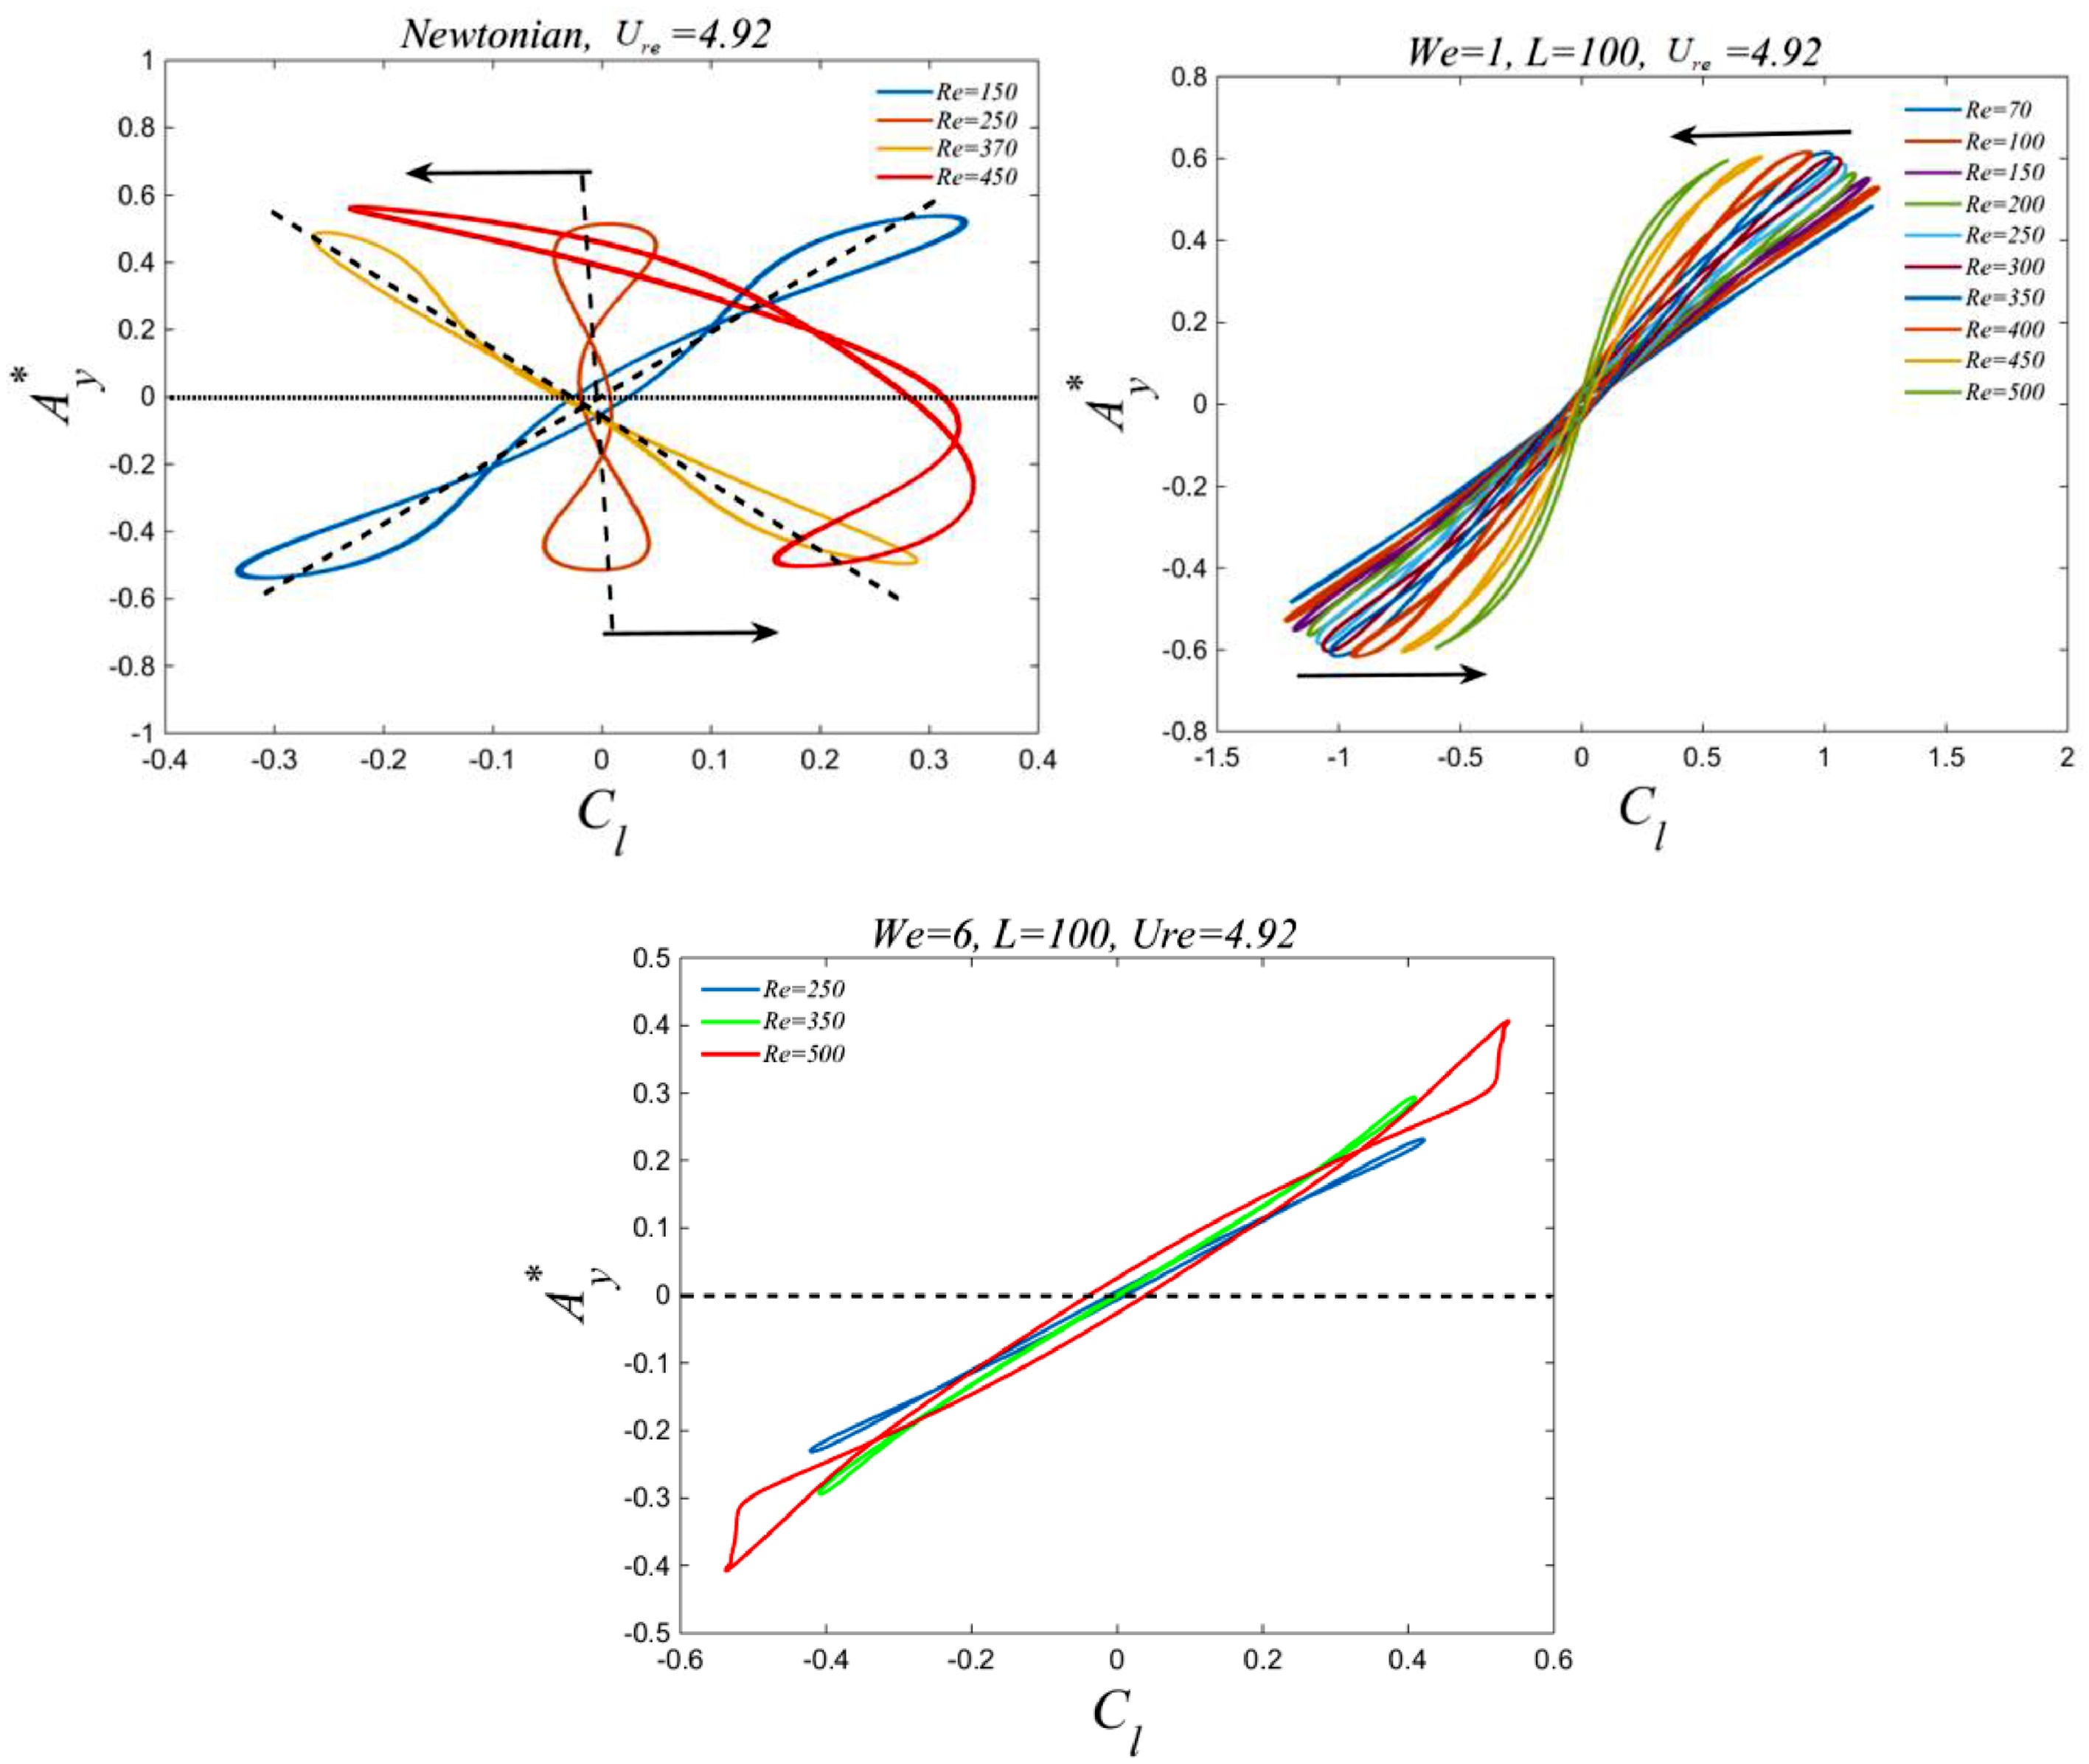
\includegraphics[width=11cm]{fig13.jpg}
    \caption{
        不同情况下振动幅度和升力系数的相位图
    }
    \label{fig:13}
\end{figure}

\begin{figure}[htbp]
    \centering
    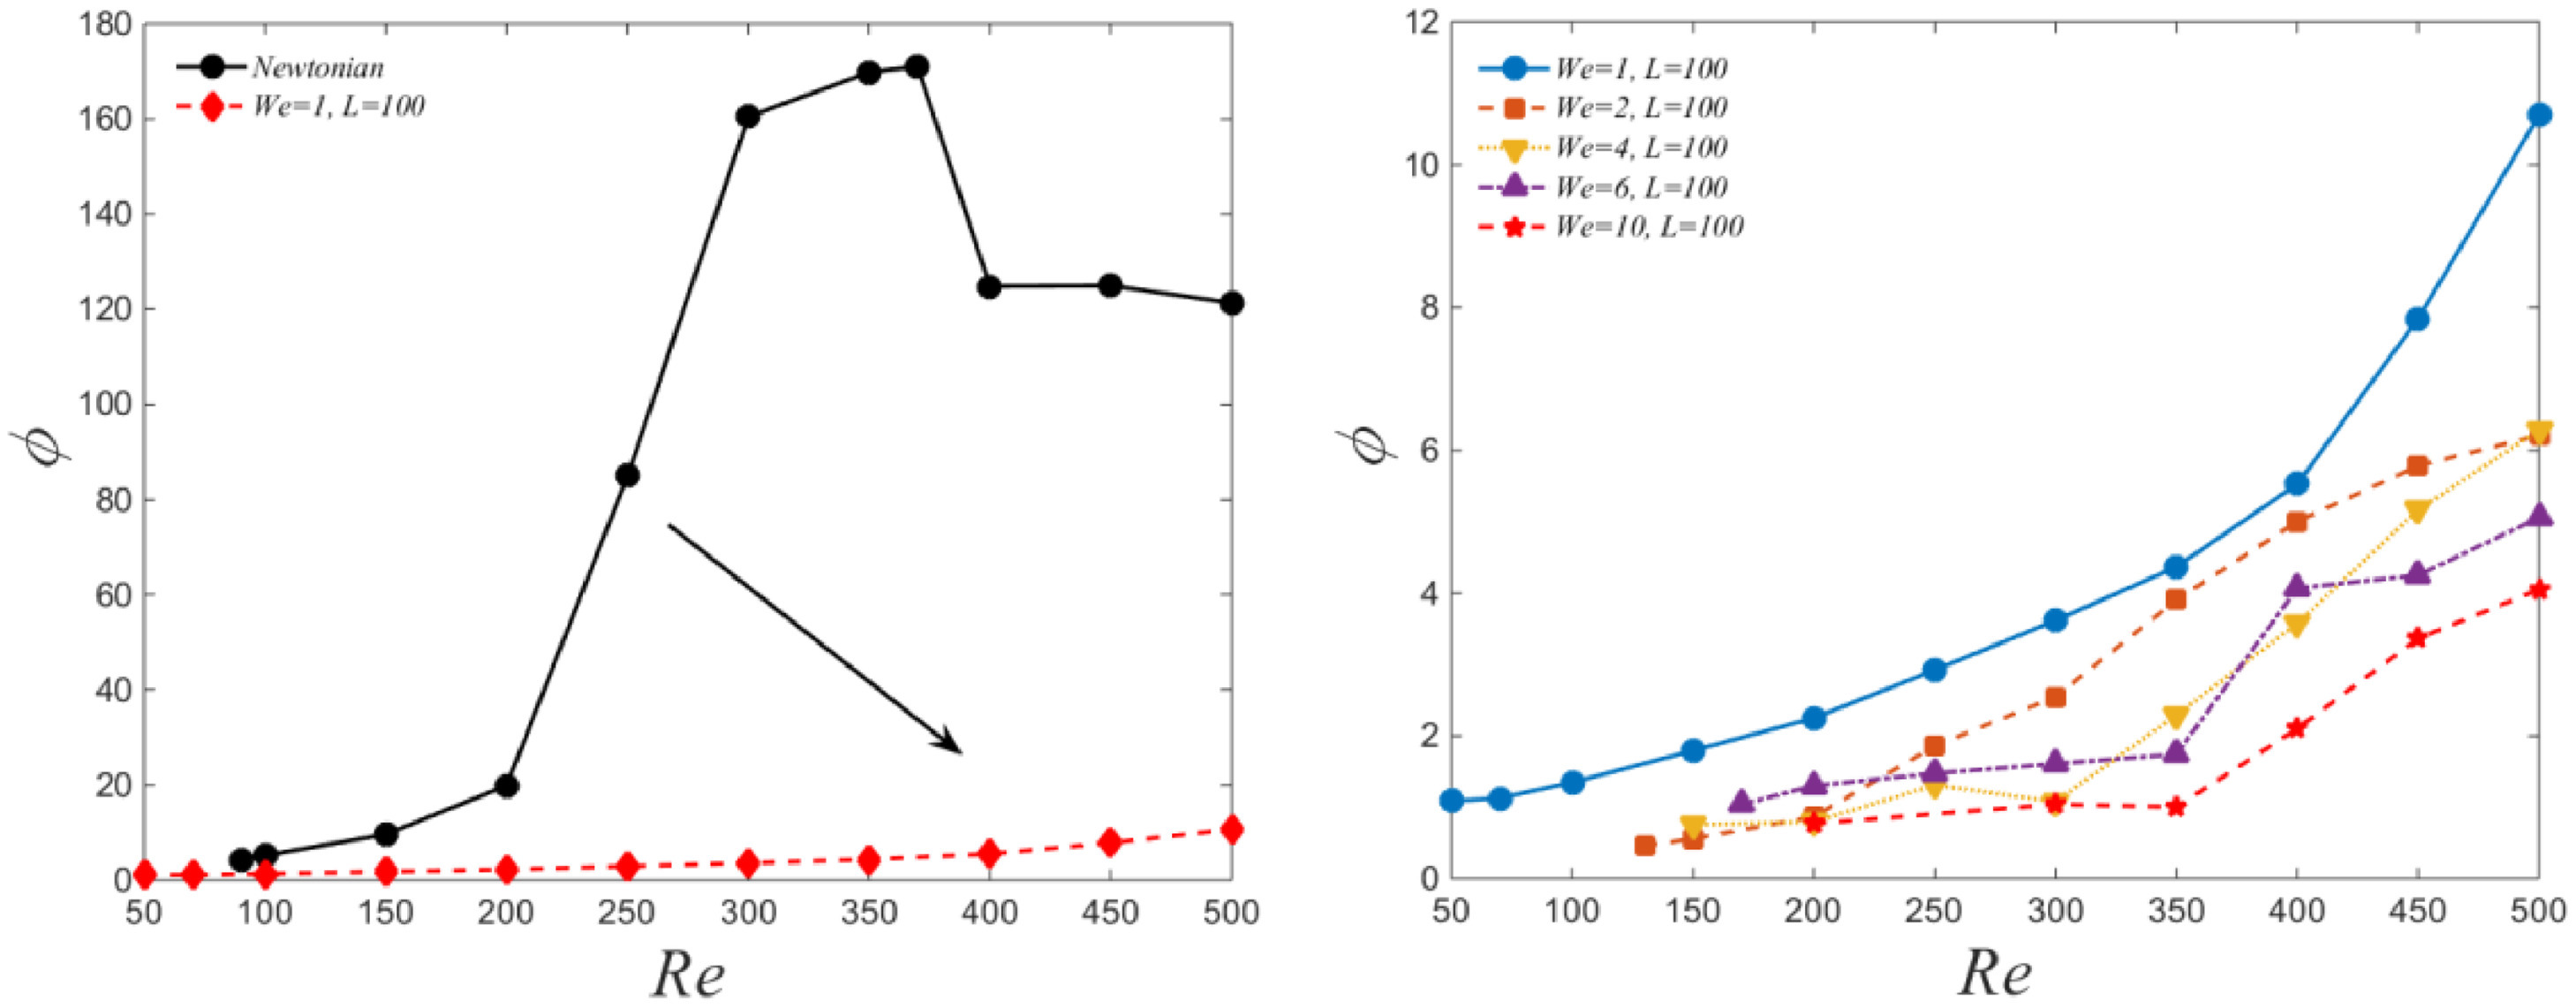
\includegraphics[width=11cm]{fig14.jpg}
    \caption{
        不同情况下振动幅度和升力系数之间的相位差异
    }
    \label{fig:14}
\end{figure}

\begin{figure}[htbp]
    \centering
    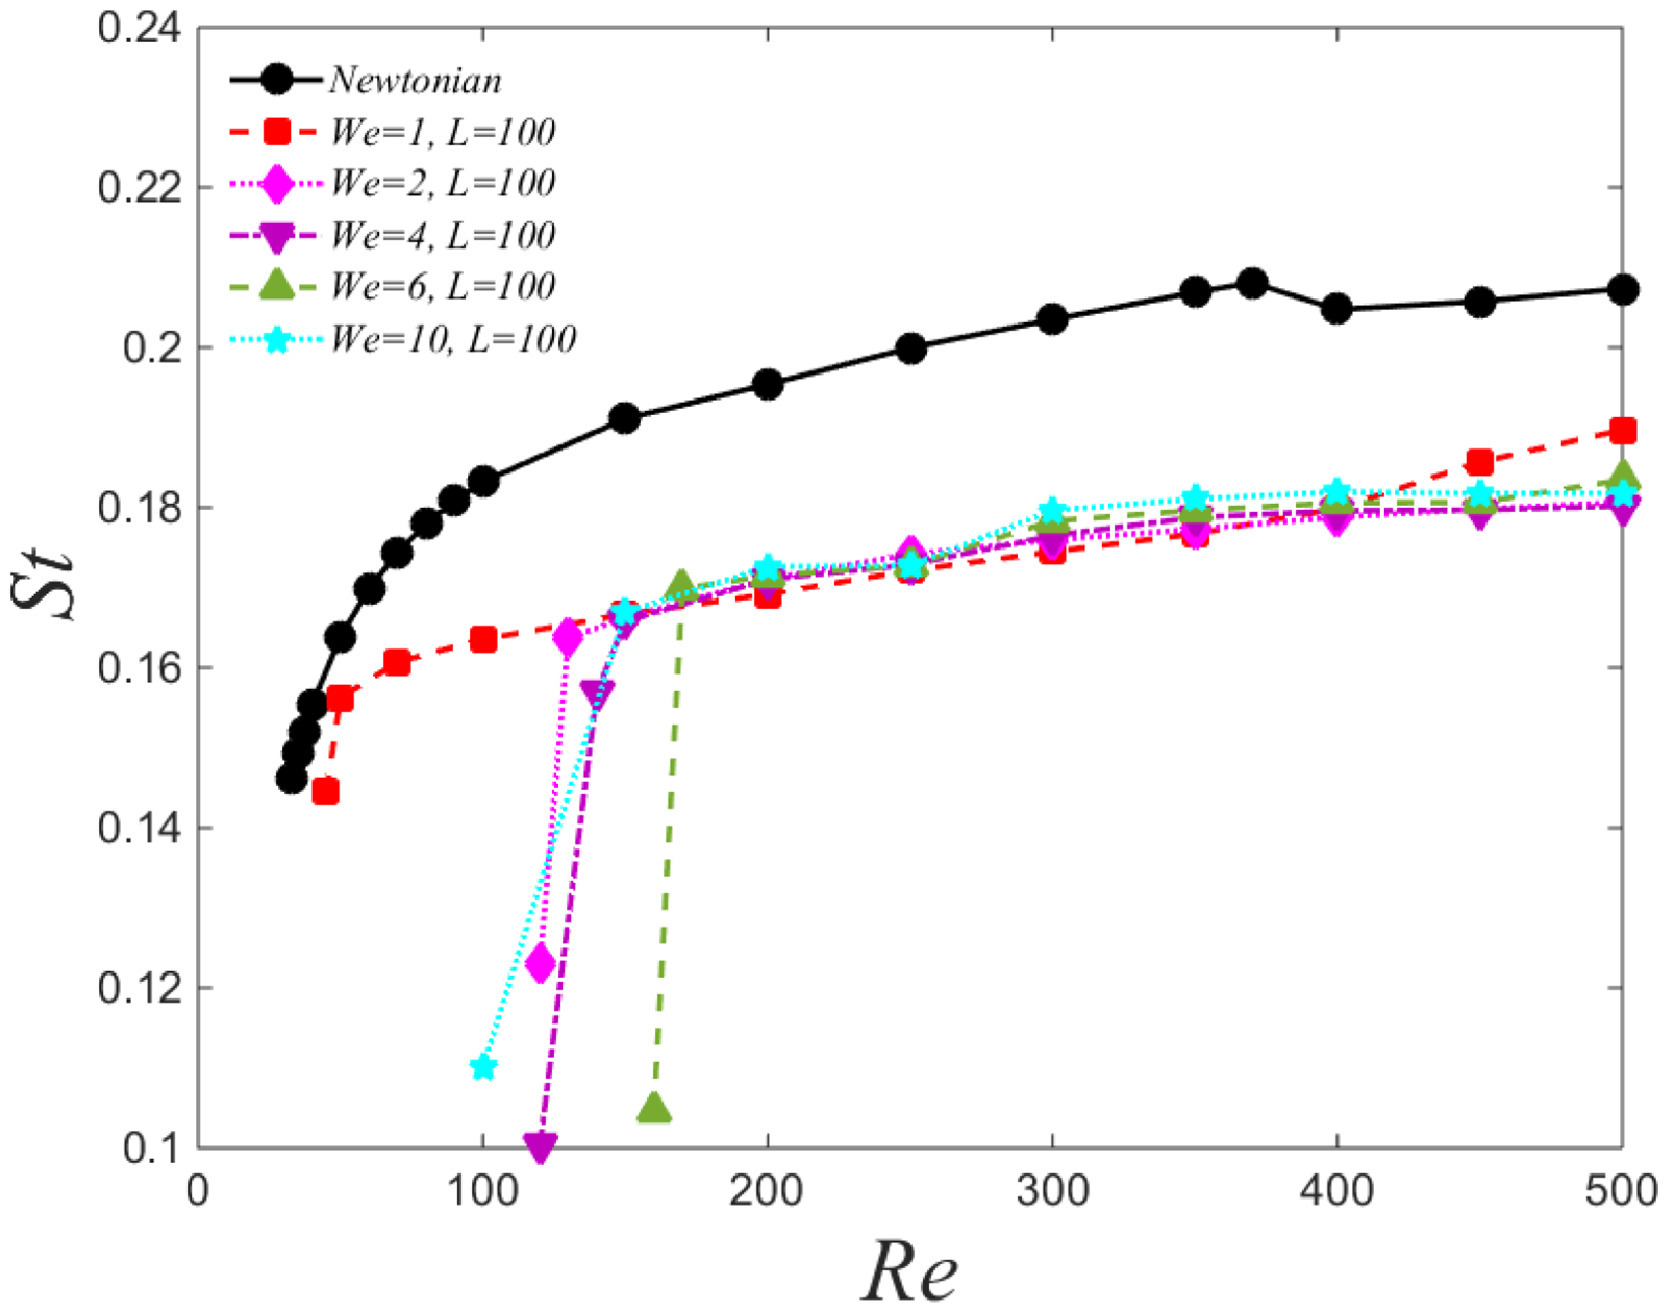
\includegraphics[width=7cm]{fig15.jpg}
    \caption{
        在减速速度为4.92时,不同情况下的St
    }
    \label{fig:15}
\end{figure}


为了理解振幅与升力系数之间的关系,
绘制了不同雷诺数下牛顿流体和粘弹性流体的振幅和升力系数的时间历史图,
分别在图\ref{fig:11}和图\ref{fig:12}中展示。
图\ref{fig:11}显示了雷诺数为150、250、370和450时牛顿流体的时间历史,
而图\ref{fig:12}则展示了雷诺数为250、350和500时粘弹性流体的时间历史。
由于升力和圆柱振动通过它们的相角紧密相关,
所以在图\ref{fig:13}中绘制了振动和升力系数的相位图,
并在图\ref{fig:14}中绘制了牛顿流体和粘弹性流体的振动和升力系数的相位角。


对于牛顿流体,清楚地看到在Re = 150时,
升力系数和圆柱振动几乎以相同的速率变化(图\ref{fig:11})。
在图\ref{fig:13}中,
可以看到振荡和圆柱升力的相位几乎分布在x = y的线附近。
在图\ref{fig:14}中,
可以看到圆柱振动和升力系数之间的相位差约为10度。
然而,观察到在Re = 250时,
当圆柱达到最大振幅位置时,
相应的升力系数几乎为零,如图\ref{fig:11}所示。
在图\ref{fig:13}中,
观察到圆柱振动和升力系数的相位几乎沿着x = 0的两侧分布。
实际上,如图\ref{fig:14}所示,
在Re = 250时,
圆柱振动和升力系数之间的相位差约为85度。
对于Re = 370的牛顿流体情况,
可以观察到升力系数和振动几乎没有同步变化,
并且相位差约为170度。
对于Re = 450的牛顿流体情况,
升力系数在时间历史上没有正负对称性,
如图\ref{fig:11}和13所示,
它们的相位差约为125度,如图\ref{fig:14}所示。
因此,升力系数与振动的关系从正相关变为负相关随着雷诺数的增加。
它们的相位差随着雷诺数的增加而增加,直到Re = 370,然后减小。

相较于牛顿流体,
在粘弹性流体中,
振动幅度与圆柱升力的相位关系非常不同。
图\ref{fig:12}描述了粘弹性流体中
Re = 250、350、500情况下圆柱的振动和升力系数的时间历史。
观察到圆柱的升力系数和振动几乎以相同的相位变化。
图\ref{fig:13}显示了不同雷诺数下升力系数和振动的相位图。
对于We = 1,随着雷诺数的增加,
振动和升力系数的相位图逆时针旋转,
从x = y附近开始。
在图\ref{fig:14}中,
相位角逐渐增加,
但随着雷诺数的增加保持在相对较低的水平。
同样,对于较高的Weissenberg数值,
相位角随着雷诺数的增加逐渐增加,
但保持在相对较低的水平,如图\ref{fig:13}和14所示。

正如前面提到的,在粘弹性流体中,升力系数
与圆柱的振动呈正相关关系,
当减速速度为4.92时。与此同时,
随着Weissenberg数值的增加,流场明显改变。
为了回答为什么升力系数与圆柱振动的相位差保持在较低水平的问题,
绘制了不同雷诺数和Weissenberg数值下的St数,
如图\ref{fig:15}所示。
观察到St数总体上随雷诺数的增加而增加,
无论是在牛顿流体还是粘弹性流体中。
对于牛顿流体,St数最终稳定在0.2左右。
但对于粘弹性流体,
St数最终达到约0.18。
当圆柱在雷诺数为3900时处于静止状态时,Richter等人
在牛顿流体中获得的St数为0.211,
在粘弹性流体中为0.189。
这表明添加聚合物会降低尾流中的频率。
相应地,圆柱在聚合物溶液中也以更低的振动频率振动。

\begin{figure}[htbp]
    \centering
    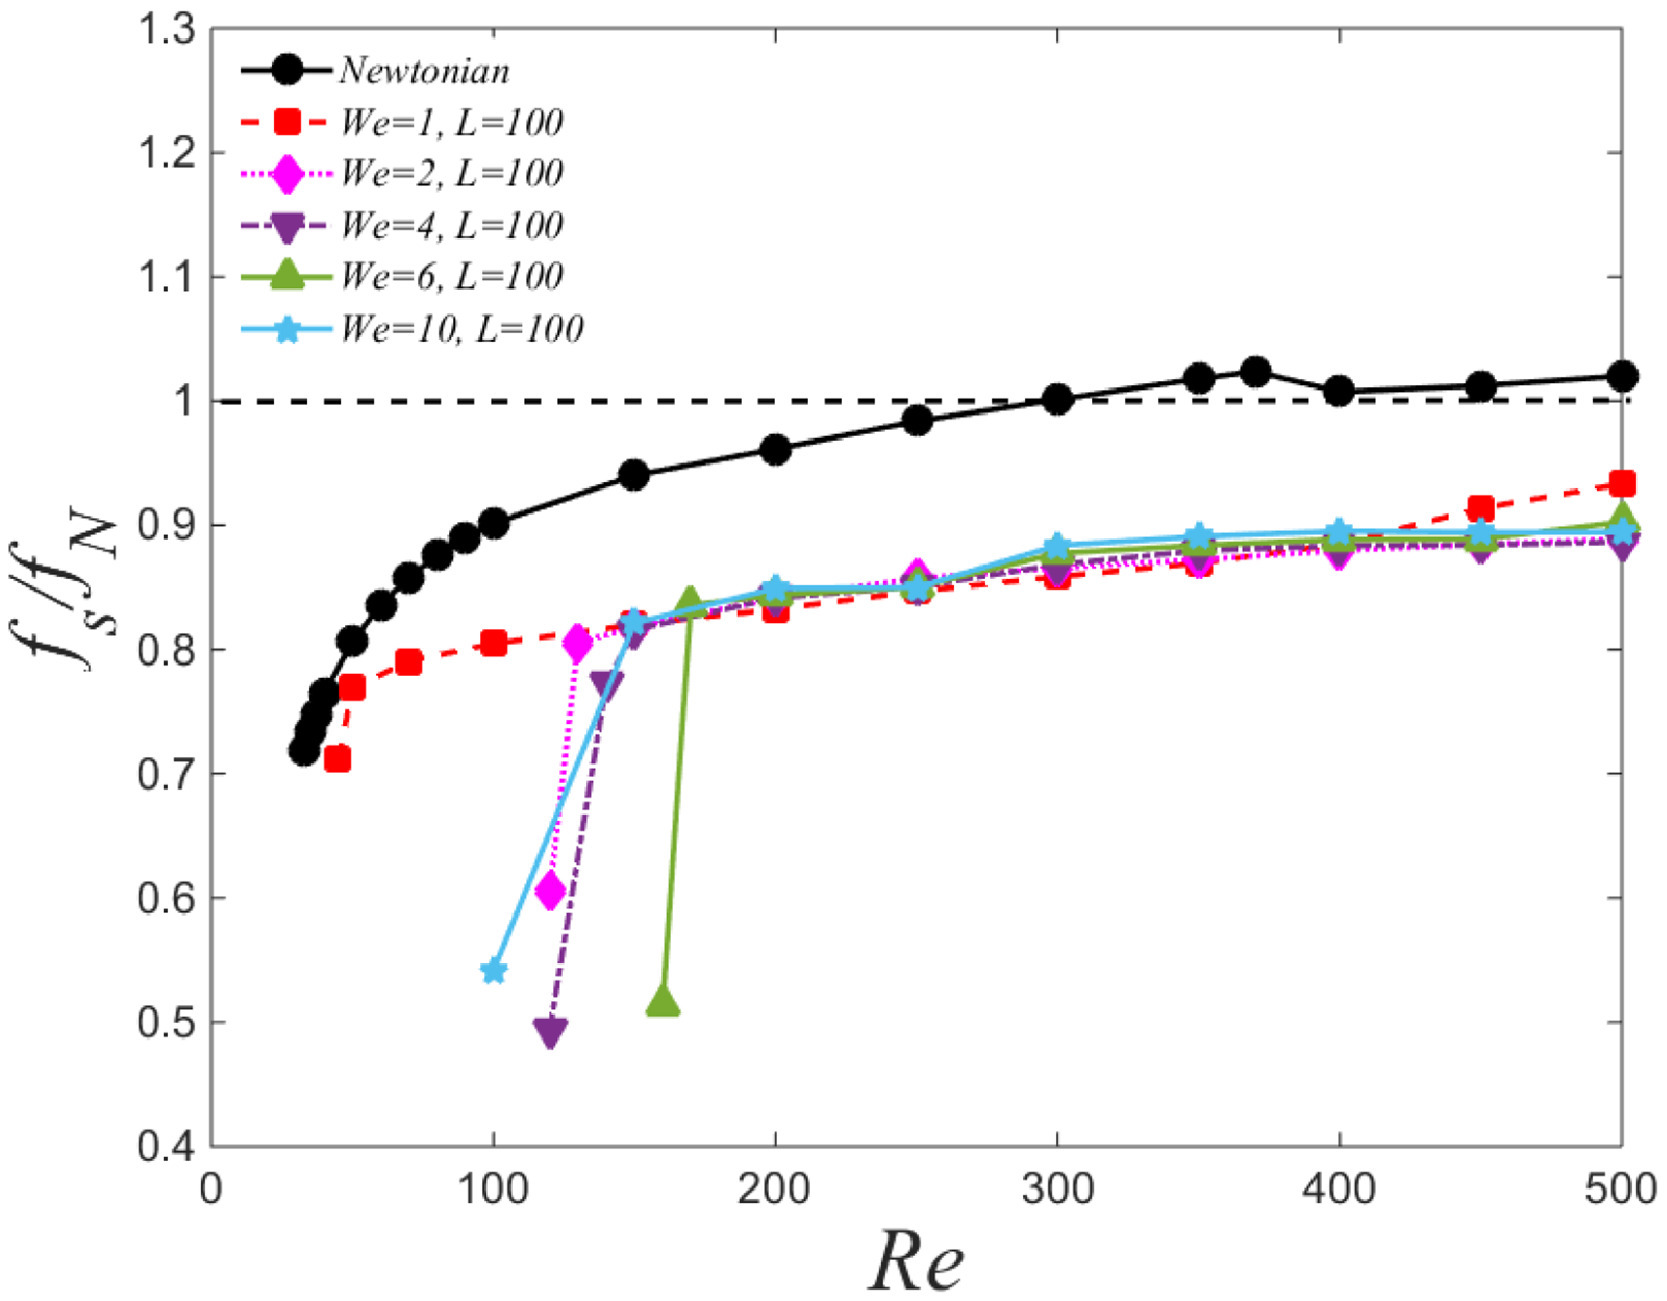
\includegraphics[width=7cm]{fig16.jpg}
    \caption{
        在减速速度为4.92时,不同情况下的振荡频率和固有频率的比值
    }
    \label{fig:16}
\end{figure}

\begin{figure}[htbp]
    \centering
    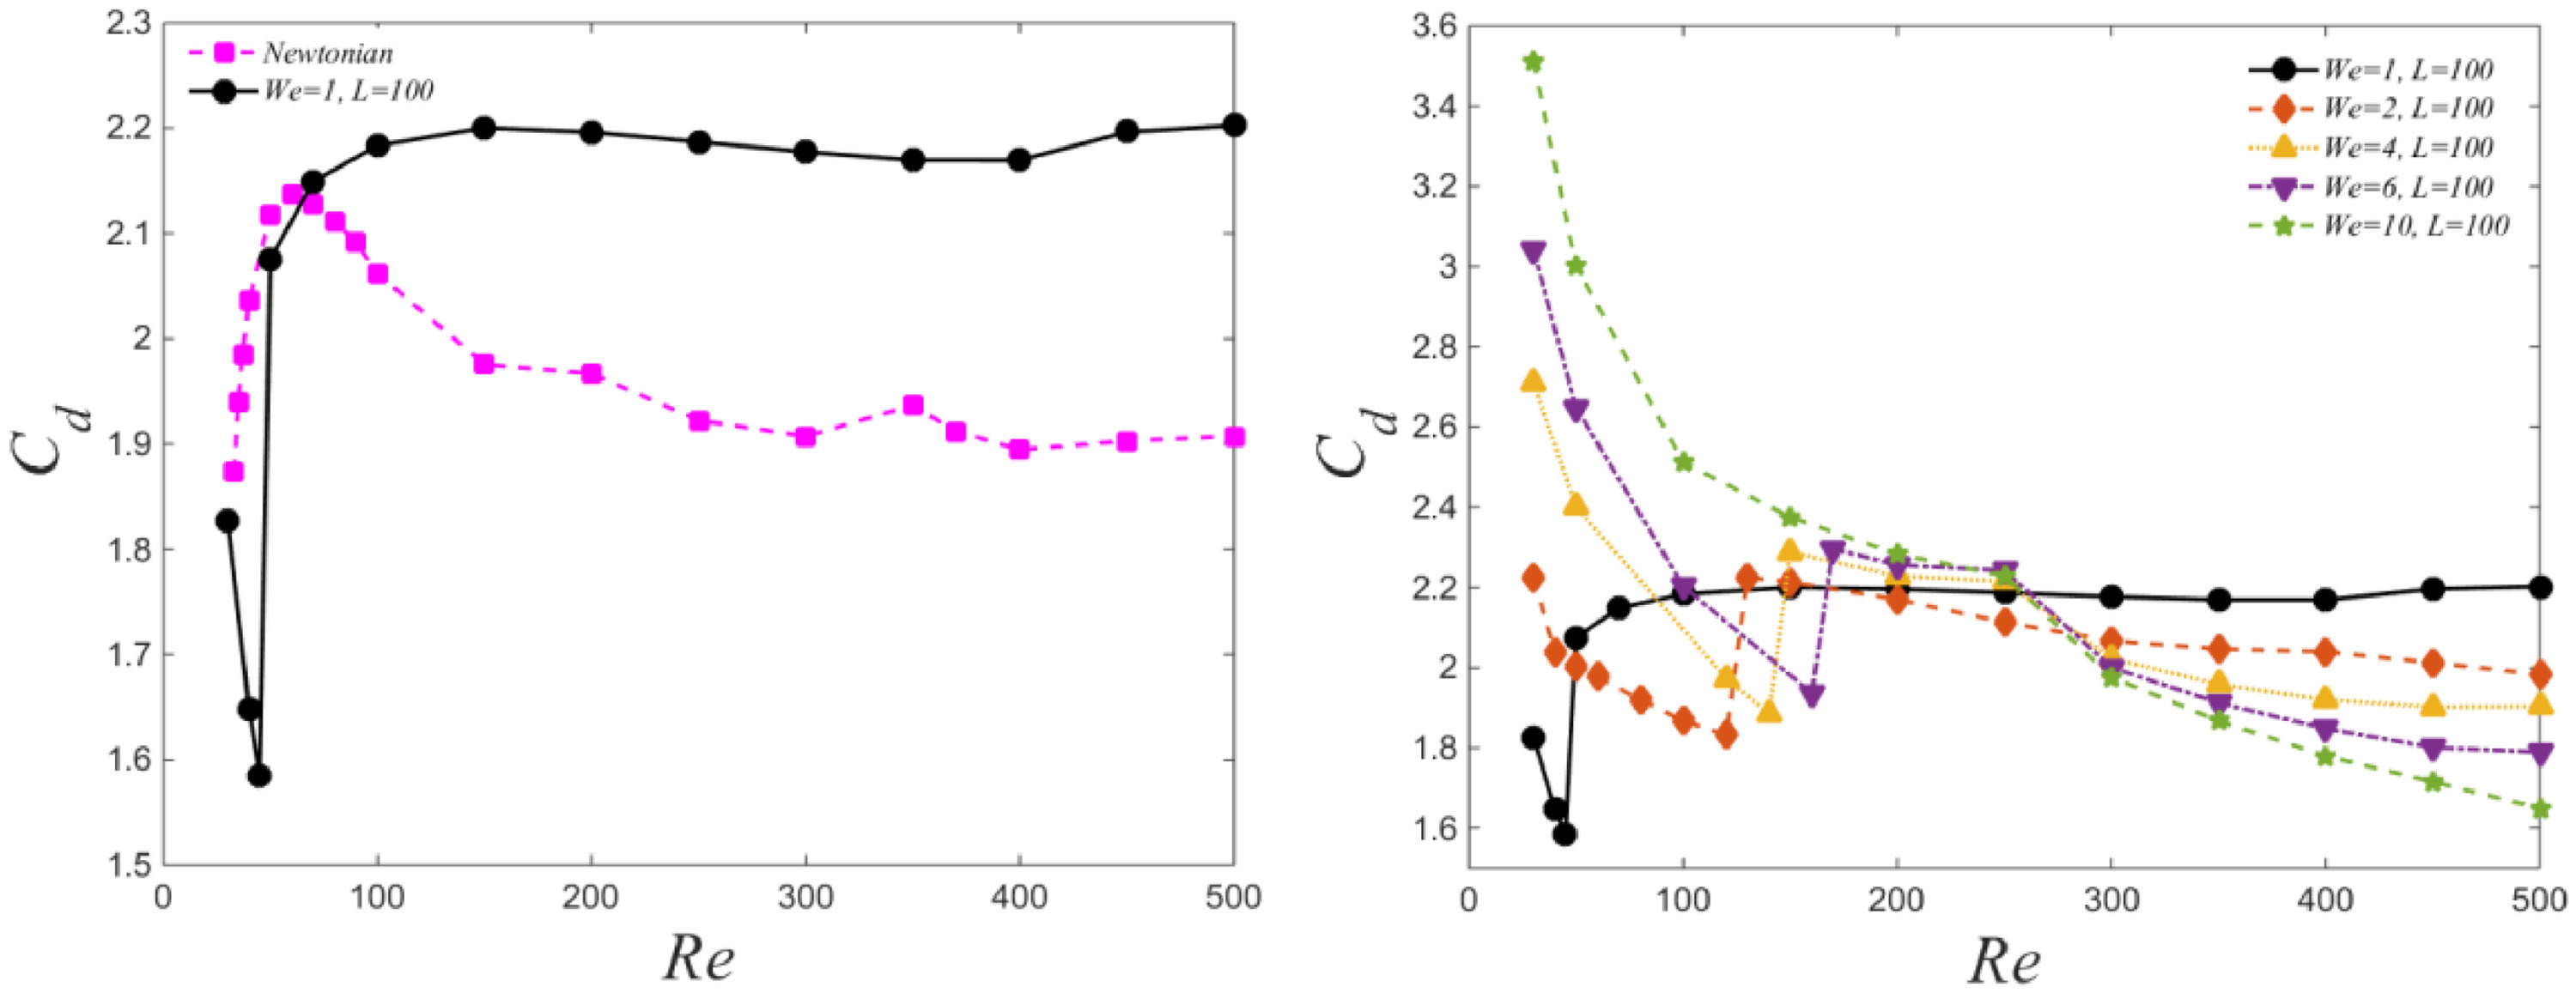
\includegraphics[width=11cm]{fig17.jpg}
    \caption{
        在减速速度为4.92时,不同情况下时间平均阻力系数
    }
    \label{fig:17}
\end{figure}

图\ref{fig:16}显示了不同雷诺数和Weissenberg数值下尾流频率与结构固有频率的比值。
对于牛顿流体,当雷诺数较大,大于300时,该比值接近于1。
关于这个比值,许多先前的研究指出,
由非稳定尾流流动引起的升力与结构振动有很大的相位差。
然而,对于粘弹性流体,尾流与结构固有频率的最大比值仅为0.933。
这是因为聚合物的添加降低了尾流的频率。
在这些情况下,圆柱的升力系数与振动之间的相位差应该保持在非常低的水平,
以便圆柱的升力能够促进其振动。
因此,在粘弹性流体中,牛顿流体中的“锁定”范围不再存在。
粘弹性流体对“锁定”范围的影响将在未来的研究中进行探索。
与图\ref{fig:16}相关的“锁定”范围的一些可能的探索方向是,
对于粘弹性流体,
应进一步增加减速速度,因为粘弹性流体延迟了VIV的发生。
此外,可以尝试较低的质量比以及较低的圆柱固有频率,
因为在粘弹性流体中,升力和涡脱落频率都会降低。

图\ref{fig:17}显示了在减速速度为4.92
时不同雷诺数和Weissenberg数值下的时间平均阻力系数。
对于牛顿流体,阻力系数在开始时随着雷诺数的增加而增加,
因为VIV倾向于增加有效阻力系数。当圆柱响应振幅达到最高值后,
阻力系数随着雷诺数的增加而减小。
在We = 1和L = 100的情况下也可以观察到类似的现象。
在粘弹性流体中,几乎所有情况下的时间平均阻力系数都高于牛顿流体。
在圆柱开始经历更大振荡之前,Weissenberg数的增加会增加阻力系数。
随着雷诺数的增加,阻力系数逐渐减小,并在临界雷诺数处经历阻力增强,
此时圆柱响应振幅急剧增加。
然而,在We = 10的情况下,阻力系数的增加过程缺失,
这是因为在当前Weissenberg数下,
振幅的增加并没有随着雷诺数的增加而急剧增加。

图\ref{fig:18}展示了在雷诺数为150、减速速度为4.92的条件下,
牛顿流体和粘弹性流体中静止和振动圆柱的升力系数和圆柱壁上的压力系数分布的时间历史。
需要注意的是,
VIV中圆柱的最终振动行为有时会依赖于初始条件和振动历史,
在较低的雷诺数范围内有相当狭窄的减速速度范围内。
在本研究中,由于重点是研究粘弹性特性对VIV的影响,
因此未研究初始条件的影响。
采用了零弹性应力和压力的均匀流场初始条件,
以及均匀的入流速度。
瞬时升力系数主要取决于圆柱上下壁之间的压力差。
对于牛顿流体中的振动圆柱
圆柱壁上的压力分布明显不同于固定圆柱,
特别是在圆柱末端,如图\ref{fig:18}所示。
在圆柱末端,由于圆柱在该时刻也向上运动,
上壁的压力较高。因此,振动圆柱的升力系数比固定圆柱小。
牛顿流体在减速速度为4.92的情况下还包括启动部分的升力系数。
相比其他情况,它需要较短的时间才能实现周期行为。
显然,在We = 10的情况下,圆柱前部的压力系数为2.1,
约为牛顿流体中的两倍,无论圆柱是固定的还是柔性的。
当圆柱静止时,可以观察到壁面上的压力在上下壁上几乎对称。
但当圆柱振动时,上下壁之间的压力差增大。


\begin{figure}[htbp]
    \centering
    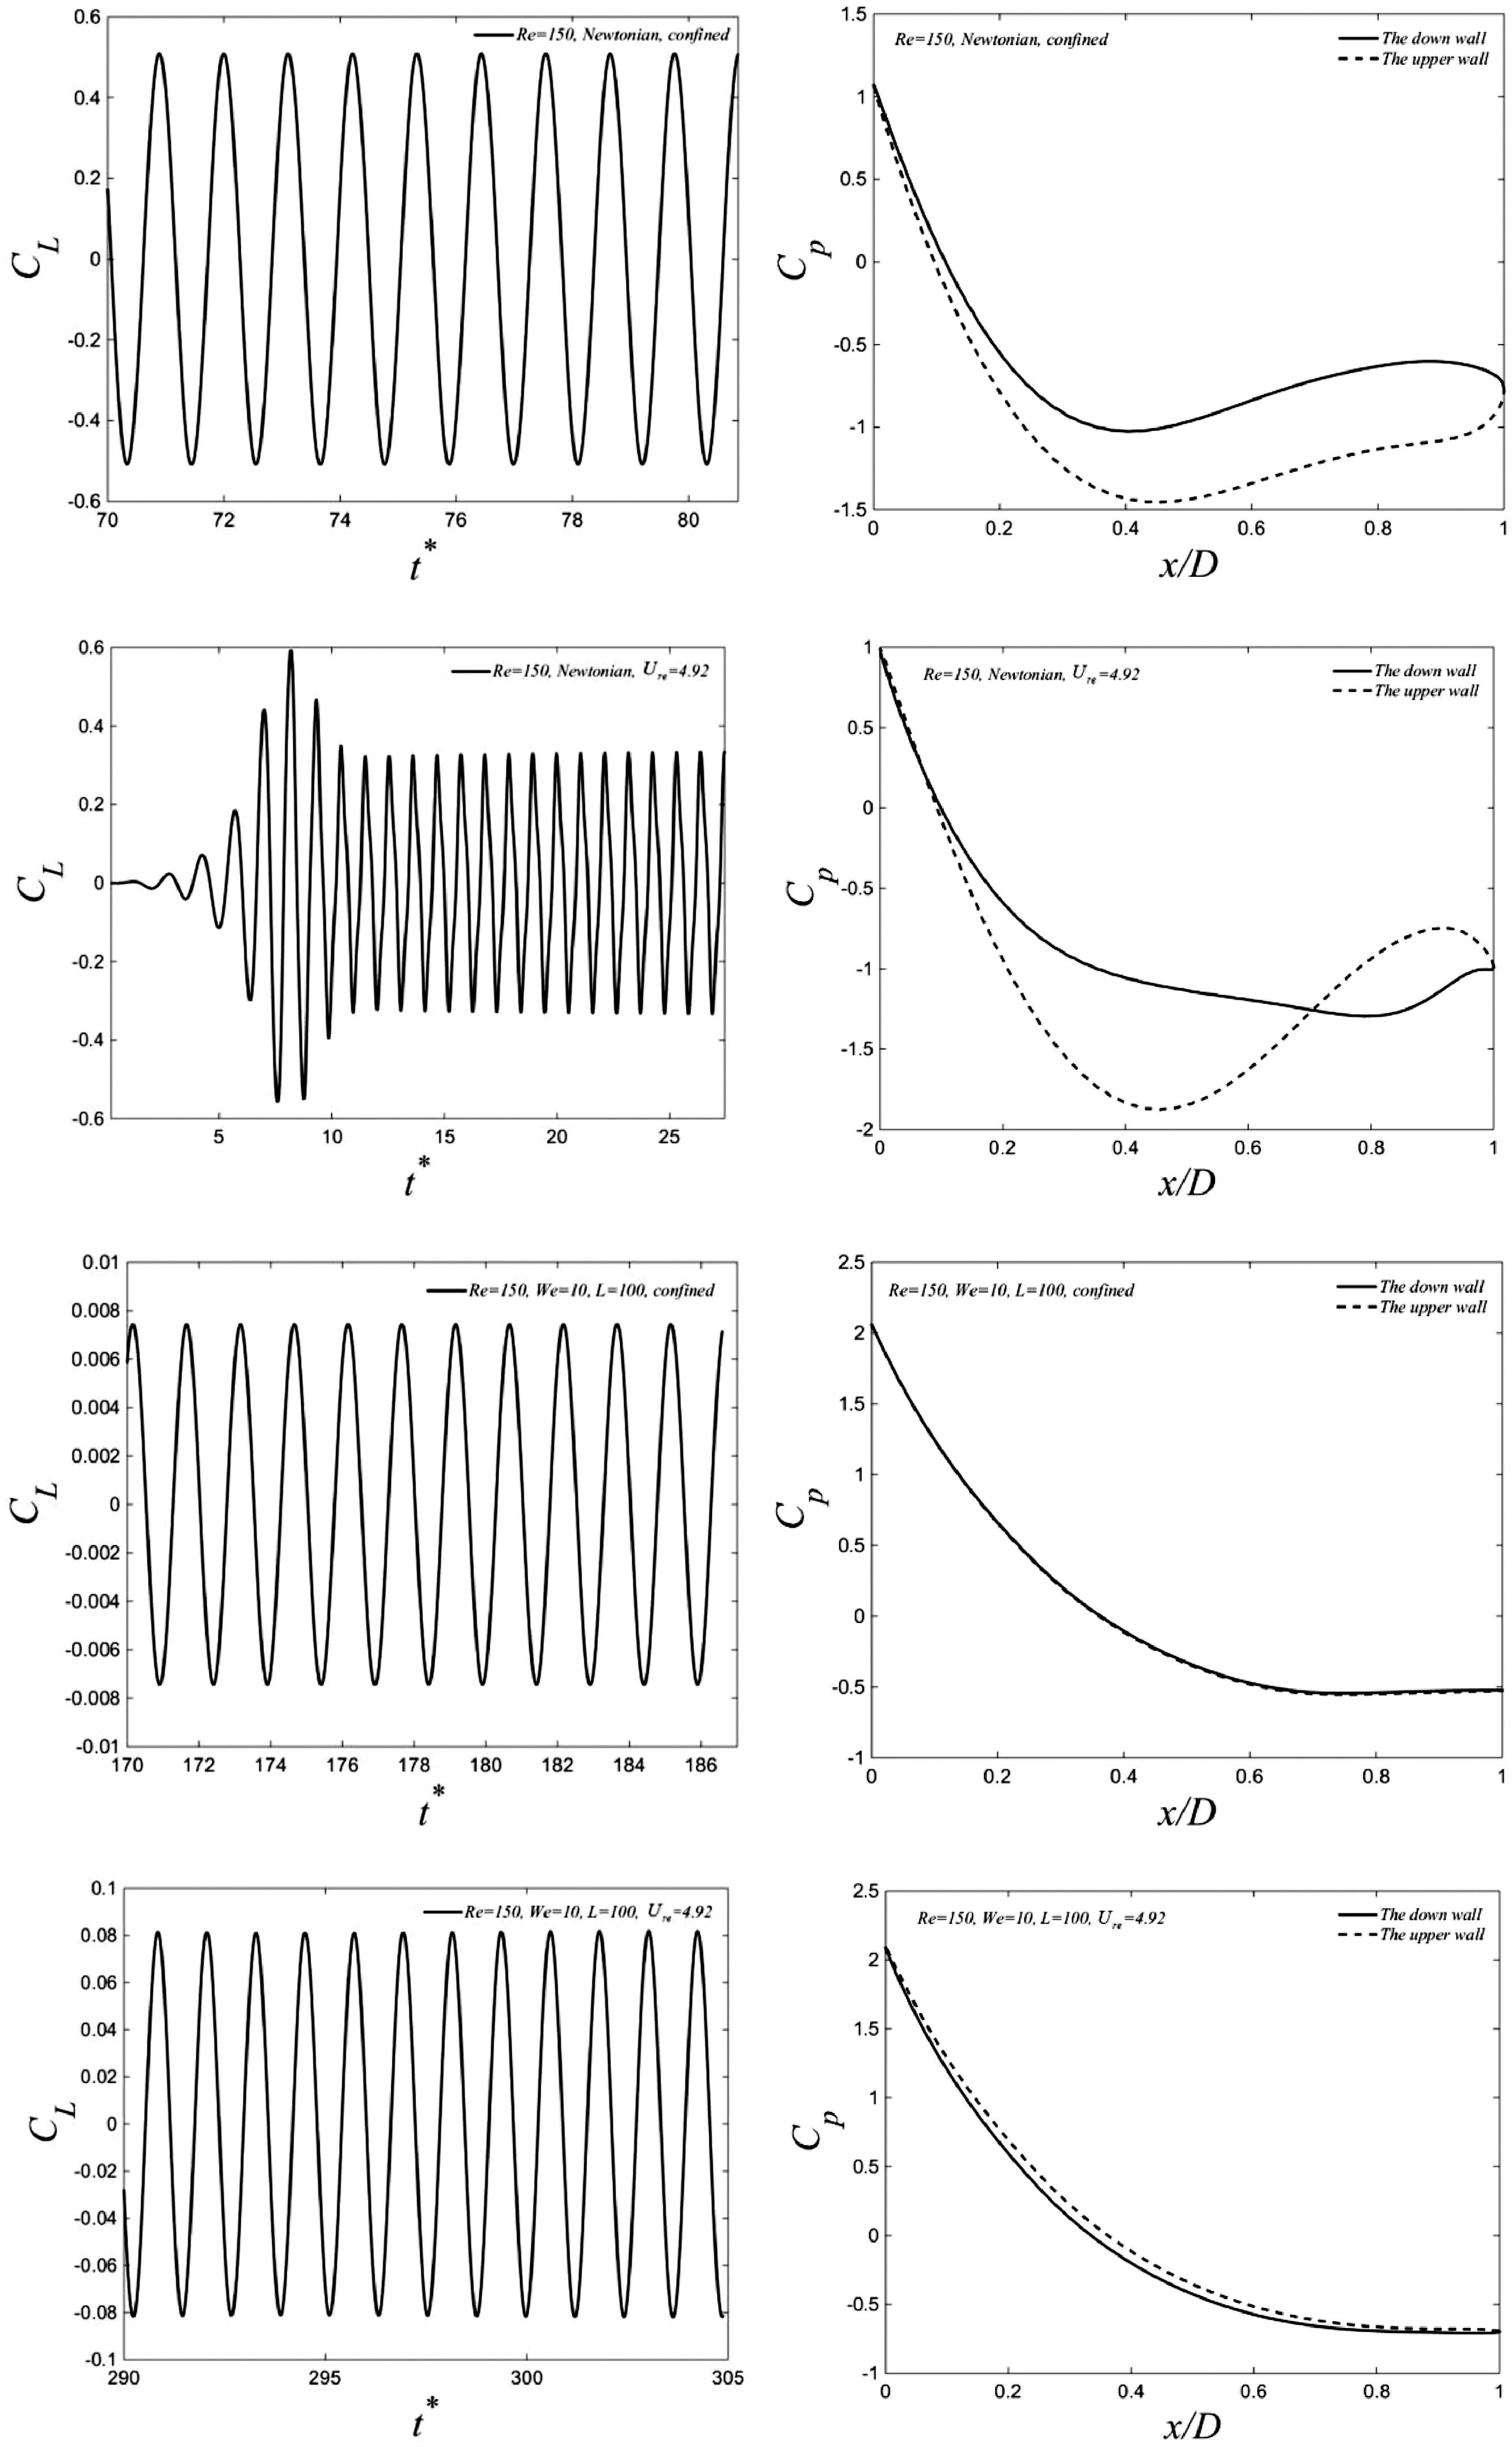
\includegraphics[width=11cm]{fig18.jpg}
    \caption{
        固定圆柱和柔性圆柱在减速速度为4.92时的升力系数和沿圆柱壁的压力系数分布的时间历史。
        对于所有情况,雷诺数均为150,而在粘弹性流体情况下,
        We = 10和L = 100。时间通过结构的固有频率进行归一化
    }
    \label{fig:18}
\end{figure}

\section{结论}

在这项研究中,
本文进行了充分的数值模拟,
研究了牛顿流体和粘弹性流体中的涡致振荡(VIV)现象。
据本文所知,这是首次提出使用聚合物添加剂来控制VIV并研究粘弹性流体对VIV的影响。
本文研究了不同流变学参数(如Weissenberg数和聚合物最大伸展性)
对减速速度相图中的圆柱响应幅值的影响。
之前对静止圆柱的涡脱落尾流的研究表明,
通过引入流体的粘弹性可以降低涡脱落频率和升力。
本文的VIV研究显示,添加聚合物通常可以抑制结构的振动。
随着Weissenberg数或聚合物最大可伸展性的增加,
抑制效果增强。
与牛顿流体相比,
粘弹性流体中的圆柱尾流振荡随着Weissenberg数的增加而减弱,
这类似于静止圆柱尾流,从而减小了圆柱的振幅。
此外,峰值振动幅值所对应的减速速度随着Weissenberg数的增加而增加,
这是由于粘弹性流体中非稳定尾流的频率降低。

尽管对于牛顿流体而言,
雷诺数对VIV的影响不如减速速度重要,
但在粘弹性流体中,
雷诺数似乎扮演着更重要的角色。
首先,在圆柱开始振动时,无论是牛顿流体还是粘弹性流体都存在临界雷诺数。
超过临界雷诺数后,
圆柱响应幅值、RMS升力系数、St数和平均阻力系数迅速增加。
在粘弹性流体中,临界雷诺数随着Weissenberg数的增加而增加。
其次,在粘弹性流体中,与牛顿流体相比,
圆柱响应的振幅更多地取决于雷诺数,尤其是当Weissenberg数较高时。
当Weissenberg数较高时,
圆柱响应振幅在临界雷诺数附近的变化不像在低Weissenberg数
下的牛顿流体或粘弹性流体那样明显,
因为非稳定尾流不像牛顿流体中那样稳
定。在粘弹性流体中,临界雷诺数附近的尾流与牛顿流体中的尾流显著不同。
在亚临界区域,横向涡团较不紧凑,
其形成区域从圆柱延伸得更远,这类似于粘弹性流体中固定圆柱的流动。
在临界雷诺数以上,
圆柱后方涡团的形成区域比之前短得多。
然而,粘弹性流体中的圆柱后方涡团与牛顿流体中的涡团明显不同,
表现为明显分层和明显拉伸的涡团沿着剪切层区域的方向延伸。

此外,本文还分析了牛顿流体和粘弹性流体中在减速速度为4.92时的升力和圆柱振动之间的相位差。
对于牛顿流体,
升力系数和圆柱振动之间的相位差随着雷诺数的增加而有很大变化。
当雷诺数大于300时,尾流的涡脱落频率与结构的固有频率近似相等。
随着雷诺数的增加,
响应幅值和升力系数之间的相位图从第一和第三象限的分支转移到第二和第四象限的分支,
导致振幅减小。
在粘弹性流体中,由于聚合物的添加,
非稳定尾流的频率降低。
当雷诺数较大时,St数达到0.18,低于所研究的结构的固有频率。
圆柱的振动与升力系数之间的相位差非常小。
聚合物的添加可以抑制非稳定尾流,同时也抑制结构的振动。

\section{感受与思考}

本文研究的是粘弹性流体的绕流问题,同时涉及了涡脱落和流固耦合问题(VIV)。
在看到这个研究问题时,我首先的一个直觉是,对于这样一个耦合问题,
在流体系统中假如含有“弹性”的本构,相当于在一个振动系统里面
改变了弹性部分的结构(而牛顿流体不考虑动能项,剪切力带来的只有阻尼部分)。
这样,至少线性意义上,流固耦合系统的能量添加了一个
流体中的弹性势能,这样势必会改变系统的固有频率。本文的数值结果
验证了这个猜测,图\ref{fig:16}清晰展示了,在较大
雷诺数下,牛顿流体振荡频率就是圆柱固体系统的固有频率;而
粘弹性流体会造成振荡频率出现变化,与固体系统的频率不同。

本文的研究方法相当于对于理想的参数设置做了一系列实验。
采用数值模拟代替实验的好处是能充分满足假设的条件以及参数
选择更加自由。同时数值模拟容易获取流场数据。当然这样不足的
就是对粘弹性本构需要进行假设,好在聚合物粘弹性流体的
本构研究已经较多,而且求解模型、数值方法都有较好的验证过程,
这样数值结果就有一定的可信度。

本文结果中最为直观的就是图\ref{fig:7}中尾迹涡量的对比,
可以看到相对于牛顿流体,粘弹性流体的尾迹分层更加明显,
而且结构更加复杂。至于为什么加入粘弹性本构后,
尾迹的涡脱落和圆柱的振荡都得到了抑制,本文是通过
提取频率、升阻力系数和振荡的波形等进行对比,
发现这与尾流震动的幅值-升力相位差、尾流脱落涡的稳定性
等都有关系。从机理的角度上讲,本文给出的数值分析结果
似乎还不是特别能够确切理解,个人感觉更多是经验上的分析
结论。

本文研究的粘弹性流体VIV问题,虽然只有较小的雷诺数,以及
很简单的几何设置和流固耦合设置,其产生的流动现象
也比相应的牛顿流体涡脱落复杂很多,这显示了非牛顿
流体本构造成复杂性的极大潜力。粘弹性的增加,从流动控制的
角度上讲,似乎可以理解为相对于牛顿流体,
增加一些基于振荡状态的被动的控制方法。

从实用角度上讲,
随着聚合物添加的增加,虽然阻力系数不一定有改善,但是
结构振荡可以得到较好的抑制,如本文所述这或许在
一些工业设备中有应用的前景。

本文的研究还是纯数值上的研究,根据其数值设定,似乎不难搭建
相应的实验环境,所以我认为最好寻求在实验中证实本研究的发现。
较为粗浅的实验设置,大概就是使用水槽或者水洞,
在其中浸入柔性支撑的圆柱进行流动实验,同时改变不同的
聚合物添加比例调节We以观察结果;不需要流动显示或者测量就可以直接
通过圆柱的振荡频率、升阻力情况与数值结果对照;也可以考虑
PIV等速度场测量方法来获取尾迹的情况,更好理解实验与数值结果的差异。

另外一方面,更大雷诺数的模拟或许也有一定意义,因为牛顿流体
会在更大雷诺数下转捩为湍流,壁面流动发生明显变化,此时的状态下
增加粘弹性本构,或许会有新的流动现象产生。当然,问题在于这样的计算
是三维的,计算消耗较大;且对牛顿流体的湍流现象的分析依然是开放话题,
增加粘弹性如何分析影响也是较大难题。


\bibliography{refs}{}
\bibliographystyle{unsrt}
































% \section{SECTION 节}

% 一个

% \subsection{SUBSECTION 小节}

% 示例

% \subsubsection{SUBSUBSECTION 小节节}

% 字体字号临时调整:
% {
%    \sffamily\bfseries\zihao{3} 哈哈哈哈哈 abcde %三号 sans系列字体(一开始设置的) 加粗
%    %只对大括号范围内的后面的字有用,在标题、题注里面同样
% }
% { 
%    \CJKfamily{kaiti}\zihao{5}\itshape 哈哈哈哈哈 abcde%三号 kaiti(一开始设置的, 斜体(英文有变)
%    %只对大括号范围内的后面的字有用,在标题、题注里面同样
% }

% 一大堆一大堆一大堆一大堆一大堆一大堆一大堆一大堆一大堆一大堆
% 一大堆一大堆一大堆一大堆一大堆一大堆一大堆一大堆一大堆一大堆一大堆一大堆
% 一大堆一大堆一大堆一大堆一大堆一大堆一大堆一大堆一大堆一大堆一大堆一大堆
% 一大堆一大堆一大堆一大堆一大堆一大堆一大堆一大堆一大堆一大堆一大堆一大堆

% \begin{center}
%     居中的什么乱七八糟东西
% \end{center}


% 一个列表:
% \begin{itemize}
%     \item asef
%     \item[\%] asdf
%     \item[\#] aaa
% \end{itemize}

% 一个有序列表:
% \begin{enumerate}
%     \item asef
%     \item[\%\%] asdf
%     \item aaa
% \end{enumerate}

% 一个嵌套列表,考虑缩进:
% \begin{enumerate}[itemindent=2em] %缩进
%     \item asef \par asaf 东西东西东西东西东西东西东西东西东西东西东西东西东西东西东西东西东西东西东西东西东西东西东西东西,
%           F不是不是不是不是不是不是不是不是不是不是不是不是不是不是不是
%           \begin{itemize}[itemindent=2em]  %缩进
%               \item lalala
%               \item mamama
%           \end{itemize}
%     \item asdf
%     \item aaa
% \end{enumerate}

% \section{SECTION}

% 图片排版:

% \begin{figure}[H]
%     \begin{minipage}[c]{0.45\linewidth}  %需调整
%         \centering
%         \includegraphics[width=8cm]{RAM_O2_4660.png}  %需调整
%         \caption{第一个图}
%         \label{fig:a}
%     \end{minipage}
%     \hfill %弹性长度
%     \begin{minipage}[c]{0.45\linewidth}  %需调整
%         \centering
%         \includegraphics[width=8cm]{RAM_O4_4660.png}  %需调整
%         \caption{第二个图}
%         \label{fig:b}
%     \end{minipage}
% \end{figure}

% figure的选项为“htbp”时,会自动浮动,是“H”则和文字顺序严格一些。

% \begin{figure}[H]
%     \begin{minipage}[c]{0.45\linewidth}  %需调整
%         \centering
%         \includegraphics[width=8cm]{RAM_O2_4660.png}  %需调整
%         \label{fig:x}
%     \end{minipage}
%     \hfill %弹性长度
%     \begin{minipage}[c]{0.45\linewidth}  %需调整
%         \centering
%         \includegraphics[width=8cm]{RAM_O4_4660.png}  %需调整
%         \label{fig:y}
%     \end{minipage}
%     \caption{第三个图}
% \end{figure}

% \begin{figure}[H]
%     \centering
%     \includegraphics[width=8cm]{RAM_O4_4660.png}  %需调整
%     \label{fig:c}
%     \caption{第四个图}
% \end{figure}



% \subsection{SUBSECTION}

% 关于怎么搞表格:

% \begin{table*}[htbp]
%     \footnotesize
%     \begin{center}
%         \caption{一端力矩载荷下的结果\fontsize{0pt}{2em}} %需要学习统一设置;0代表不变?
%         \label{表2}
%         \begin{tabular}{|c|c|c|c|c|c|c|}
%             \hline
%             节点数                              & 积分方案              & 单元数                & $h=1m$                & $h=0.1m$              & $h=0.05m$             & $h=0.01m$             \\
%             \hline
%             \multirow{6}{*}{2}                  & \multirow{3}{*}{精确} & 1                     & 4.235294117647059E-08 & 1.406250000000000E-06 & 2.862823061630218E-06 & 1.439654482924097E-05 \\
%             \cline{3-7}
%                                                 &                       & 10                    & 5.975103734439814E-08 & 4.235294117646719E-05 & 1.800000000000410E-04 & 1.406249999999849E-03 \\
%             \cline{3-7}
%                                                 &                       &
%             10000                               & 5.999999915514277E-08 & 5.999996622448291E-05 & 4.799989509752562E-04 & 5.999793702477535E-02                                                 \\
%             \cline{2-7}
%                                                 & \multirow{3}{*}{减缩} & 1                     & 6.000000000000001E-08 & 5.999999999999972E-05 & 4.799999999999911E-04 & 6.000000000003492E-02 \\
%             \cline{3-7}
%                                                 &                       & 10                    & 6.000000000000071E-08 & 5.999999999999142E-05 & 4.799999999995399E-04 & 5.999999999903294E-02 \\
%             \cline{3-7}
%                                                 &                       & 10000                 & 6.000000112649221E-08 & 5.999999234537814E-05 & 4.799997501925065E-04 & 6.000037607984510E-02 \\
%             \hline

%             \multirow{6}{*}{3}                  & \multirow{3}{*}{精确} & 1                     & 6.000000000000003E-08 & 6.000000000000202E-05 & 4.800000000000831E-04 & 6.000000000056749E-02 \\
%             \cline{3-7}
%                                                 &                       & 10                    & 5.999999999999932E-08 & 6.000000000004190E-05 & 4.800000000000206E-04 & 6.000000001613761E-02 \\
%             \cline{3-7}
%                                                 &                       & 10000                 & 6.000000013769874E-08 & 5.999989495410481E-05 & 4.799942099727246E-04 & 6.000263852944890E-02 \\
%             \cline{2-7}
%                                                 & \multirow{3}{*}{减缩} & 1                     & 6.000000000000002E-08 & 6.000000000000267E-05 & 4.800000000000754E-04 & 5.999999999989982E-02 \\
%             \cline{3-7}
%                                                 &                       & 10                    & 5.999999999999899E-08 & 5.999999999987338E-05 & 4.799999999947916E-04 & 5.999999998625345E-02 \\
%             \cline{3-7}
%                                                 &                       & 10000                 & 5.999999728157785E-08 & 5.999994914321980E-05 & 4.800008377474699E-04 & 5.999472246346305E-02 \\
%             \hline

%             \multicolumn{3}{|c|}{欧拉-伯努利解} & 6.000000000000000E-08 & 6.000000000000000E-05 & 4.800000000000000E-04 & 6.000000000000000E-02                                                 \\
%             \hline
%         \end{tabular}
%     \end{center}
% \end{table*}

% 多行、多列表格的示例,基本思想是,多列的那个东西放在多列的最上面一格,下面的行要用\&来空开,也就是\&的数目
% 和普通表格一样,是列数减一;
% 多列的部分的话,就是每行内的操作,相应的\&就少了,见最后一行。

% tabular的“|c|c|c|c|c|c|c|”,意思是,竖线-居中-竖线-居中-竖线……,可以选择省略一些竖线;
% 每行之间的hline,代表贯通的横线,cline是有范围的横线。

% \subsubsection{SUBSUBSECTION}

% newcommand可以用来定义新指令,似乎基本上就是字符串替换……不太懂,总之在公式里面可以用,
% 外面也经常用。






% 公式这么写:
% \begin{equation}
%     \begin{aligned}
%         \frac{aa(x^1+x^2)}{\sqrt{x^1x^2}}
%         \nabla\times\uu
%         = & u_{j;m}\g^m\times\g^j
%         =u_{j;m}\epsilon^{mjk}\g_k
%         =u_{j,m}\epsilon^{mjk}\g_k                           \\
%         = & \frac{1}{\sqrt{g}}\left|
%         \begin{matrix}
%             \g_1       & \g_2       & \g_3       \\
%             \partial_1 & \partial_2 & \partial_3 \\
%             u_1        & u_2        & u_3
%         \end{matrix}
%         \right|
%         =\frac{\sqrt{x^1x^2}}{aa(x^1+x^2)}
%         \left|
%         \begin{matrix}
%             \g_1                        & \g_2                        & \g_3       \\
%             \partial_1                  & \partial_2                  & \partial_3 \\
%             u^1\frac{a^2(x^1+x^2)}{x^1} & u^2\frac{a^2(x^1+x^2)}{x^2} & u^3
%         \end{matrix}
%         \right|                                              \\
%         = & \frac{\sqrt{x^1x^2}}{aa(x^1+x^2)}
%         [[\g_1\,\g_2\,\g_3]]
%         diag\left(
%         u^3_{,2}-u^2_{,3}\frac{a^2(x^1+x^2)}{x^2},\,
%         u^1_{,3}\frac{a^2(x^1+x^2)}{x^1}-u^3_{,1},\, \right. \\
%           & \left.
%         u^2_{,1}\frac{a^2(x^1+x^2)}{x^2}+u^2\frac{a^2}{x^2}
%         -
%         u^1_{,2}\frac{a^2(x^1+x^2)}{x^1}-u^1\frac{a^2}{x^1}
%         \right)                                              \\
%         = & \frac{\sqrt{x^1x^2}}{aa(x^1+x^2)}
%         [[\bm{e}_1\,\bm{e}_2\,\bm{e}_3]]
%         \left[\begin{array}{ccc} a & -a & 0\\ \frac{a\,x^{2}}{\sqrt{x^{1}\,x^{2}}} & \frac{a\,x^{1}}{\sqrt{x^{1}\,x^{2}}} & 0\\ 0 & 0 & 1 \end{array}\right]              \\
%           & diag\left(
%         u^3_{,2}-u^2_{,3}\frac{a^2(x^1+x^2)}{x^2},\,
%         u^1_{,3}\frac{a^2(x^1+x^2)}{x^1}-u^3_{,1},\, \right. \\
%           & \left.
%         u^2_{,1}\frac{a^2(x^1+x^2)}{x^2}+u^2\frac{a^2}{x^2}
%         -
%         u^1_{,2}\frac{a^2(x^1+x^2)}{x^1}-u^1\frac{a^2}{x^1}
%         \right)
%     \end{aligned}
%     \label{eq:curlu}
% \end{equation}

% 如果不想带编号的公式(或者图表),用 equation* 这种环境。

% 引用,如果是引用的图表,就用表\ref{表2},图\ref{fig:a}这种,代码里是用label定义的标签来引用,
% 编号是自动生成的。公式引用一般写成:\eqref{eq:curlu}。目前这些引用自动会有超链接,反正有那个包自动
% 好像就会有……呜呜呜也不知道是怎么做到的,先这么用吧。

% \paragraph{PARA}

% 引用文献用\\cite这些,要用bibtex,暂时不做。

% \subparagraph{SUBPARA}

\end{document}